% THIS DOCUMENT IS FOLLOWS THE VOLERE TEMPLATE BY Suzanne Robertson and James Robertson
% ONLY THE SECTION HEADINGS ARE PROVIDED
%
% Initial draft from https://github.com/Dieblich/volere
%
% Risks are removed because they are covered by the Hazard Analysis
\documentclass[12pt]{article}

\usepackage{float}
\usepackage{graphicx}
\usepackage{longtable}
\usepackage{booktabs}
\usepackage{tabularx}
\usepackage{hyperref}
\usepackage{amsfonts}
\usepackage{amsmath}

\hypersetup{
    bookmarks=true,         % show bookmarks bar?
      colorlinks=true,      % false: boxed links; true: colored links
    linkcolor=red,          % color of internal links (change box color with linkbordercolor)
    citecolor=green,        % color of links to bibliography
    filecolor=magenta,      % color of file links
    urlcolor=cyan           % color of external links
}

\newcommand{\lips}{\textit{Insert your content here.}}
\newcommand{\tabitem}{~~\llap{\textbullet}~~}
\newcommand{\probP}{\text{I\kern-0.15em P}}

%% Comments

\usepackage{color}

\newif\ifcomments\commentstrue %displays comments
%\newif\ifcomments\commentsfalse %so that comments do not display

\ifcomments
\newcommand{\authornote}[3]{\textcolor{#1}{[#3 ---#2]}}
\newcommand{\todo}[1]{\textcolor{red}{[TODO: #1]}}
\else
\newcommand{\authornote}[3]{}
\newcommand{\todo}[1]{}
\fi

\newcommand{\wss}[1]{\authornote{blue}{SS}{#1}} 
\newcommand{\plt}[1]{\authornote{magenta}{TPLT}{#1}} %For explanation of the template
\newcommand{\an}[1]{\authornote{cyan}{Author}{#1}}

%% Common Parts

\newcommand{\progname}{Software Engineering} % PUT YOUR PROGRAM NAME HERE
\newcommand{\authname}{Team \#11, OKKM Insights
\\ Mathew Petronilho
\\ Oleg Glotov
\\ Kyle McMaster
\\ Kartik Chaudhari} % AUTHOR NAMES                  

\usepackage{hyperref}
    \hypersetup{colorlinks=true, linkcolor=blue, citecolor=blue, filecolor=blue,
                urlcolor=blue, unicode=false}
    \urlstyle{same}
                                


\begin{document}

\title{Software Requirements Specification for \progname: GeoWeb} 
\author{\authname}
\date{\today}
	
\maketitle

~\newpage

% \pagenumbering{roman}

\tableofcontents

~\newpage

\section*{Revision History}

\begin{tabularx}{\textwidth}{p{3cm}p{2cm}X}
\toprule {\textbf{Date}} & {\textbf{Authors}} & {\textbf{Version}}\\
\midrule
10/09/2024 & Oleg, Kyle, Kartik, Mathew & Revision 0\\

\bottomrule
\end{tabularx}

~\\

~\newpage
\section{Purpose of the Project}
\subsection{User Business}
There is currently a lack of high-quality, labeled satellite imagery datasets tailored for specific use cases. Many industries require specialized data for tasks like disaster 
response, environmental monitoring, urban planning, or defense, but building these datasets manually is time-consuming, costly, inefficient and may require expert data analysis. 
This hinders the development and deployment of accurate computer vision models for critical use cases across these various industries.

The purpose of this project is to create an online platform that accelerates this process and brings simplicity to satellite imagery data analysis.
\subsection{Goals of the Project}
\subsubsection*{High Data Accuracy}
The system should have high classification accuracy for objects reported in the images. The core problem this system must solve is extracting useful information from the provided images.
 One key metric to determine the utility of the information found, is the classification accuracy of objects identified in the images. If the system is 
 not able to determine what is contained in an image, it will not be useful to stakeholders.
\subsubsection*{Ease of use}
The system should be very easy for stakeholders to use. There should be very low friction for users to classify images and objects found
within images, with minimal training. It should also be simple for users to upload images to be analyzed. To maximize the information gained from users who are contributing to classification efforts, the system must ensure it is simple for users to 
get started with, and continue using the system. This is necessary to build a large enough user base, which will make it more likely to get insights in an acceptable 
amount of time.
\subsubsection*{Minimizing Cost to Analyze Images}
The system should minimize the cost for users request insights from images. This could be implemented through intelligent algorithms for task delegation. Users of the system who upload images are interested in getting an appropriate return for their investment. If the cost to analyze is too high, the platform will not
retain a sufficiently large user base of purchasers.
\subsubsection*{Results Returned Within Appropriate Timeframe}
The system should ensure the time it takes to obtain information from images is within a specified limit, as determined by users who upload images. Purchasers will have some time limit they require the system to process images within. To ensure timing needs are met, the system should provide realistic timelines and stick to them.
\subsubsection*{High System Reliability and Accessibility}
The system should be useable remotely for purchasers and labellers, and have minimal downtime.The system should allow purchasers to upload images without being physically located where the system is hosted to ensure flexibility of use. The same should also be true for labellers, as they 
should be able to perform their tasks remotely. In both cases, the system should have low down time as to not introduce additional friction into the completion of tasks.
\section{Stakeholders}

\subsection{Customer}
End Clients/Customers: These stakeholders include governments, NGOs, private companies, and environmental organizations that pay for access to the labeled datasets and models. They rely on these datasets to make informed decisions in areas like environmental monitoring, urban planning, or defense-related tasks. Their satisfaction depends on the accuracy and reliability of both the data and the models provided.


\subsubsection{Users (Data Labelers)}
Data labelers are a core group of users responsible for annotating and classifying raw satellite imagery. Their role is fundamental to the project as they provide the labeled data required to train AI models. Data labelers are essential to the project's workflow, bridging the gap between raw data and actionable insights for stakeholders. Their contributions not only shape the quality of the AI models but also impact the effectiveness of the end clients decision-making processes.


\subsection{Other Stakeholders}
Beyond the primary stakeholders, other key groups that benefit from high-quality satellite imagery datasets include:
\begin{itemize}
    \item \textbf{Defense Agencies:} Rely on tailored data for surveillance, intelligence, and threat detection to enhance national security.
    \item \textbf{Environmental Agencies:} Use satellite data to monitor ecosystems, track deforestation, and respond to climate change.
    \item \textbf{Urban Planners:} Leverage data to manage land use, plan infrastructure development, and promote sustainable growth in cities.
    \item \textbf{Disaster Relief Organizations:} Depend on satellite imagery to assess damage in real-time and prioritize aid during crisis situations, making these datasets crucial for effective disaster response.
    \item \textbf{Image Labeling Teams:} Manually classify and annotate satellite images. Their work is crucial for building accurate datasets, and they benefit from improved tools and clearer guidelines to make the labeling process more efficient.
\end{itemize}

\subsection{Intended Audience}

This section outlines the primary, secondary, and tertiary audiences for this document, along with the scope of knowledge assumed and its relevance for onboarding and continued project development.

\subsection{Primary Audience}
\begin{itemize}
    \item \textbf{Development Team:} This document is intended for current or future developers and engineers working on the project. It assumes a technical background in areas such as crowdsourcing platforms, satellite image processing, and AI modeling. It provides a foundation for tracking design decisions and assumptions made by the original developers, who possess expertise in data processing, backend development, and labeling systems.
\end{itemize}

\subsection{Secondary Audience}
\begin{itemize}
    \item \textbf{Project Stakeholders:} Stakeholders, including clients, NGOs, or government agencies, may refer to this document to understand technical decisions, product constraints, and the alignment with business goals.
    \item \textbf{Platform Maintenance Technicians:} The document is relevant for ensuring ongoing maintenance and troubleshooting, offering a detailed understanding of system requirements and operations.
\end{itemize}

\subsection{Tertiary Audience}
\begin{itemize}
    \item \textbf{Future Researchers or Collaborators:} Academics or collaborators interested in extending the platform’s functionality can use this document as a foundation.
    \item \textbf{QA and Testing Teams:} The functional and non-functional requirements detailed in this document can be utilized for validation and verification processes.
\end{itemize}

\subsection{Scope of Knowledge Assumed}
\begin{itemize}
    \item \textbf{For Developers:} Familiarity with web-based systems, satellite data, and crowdsourcing concepts is assumed.
    \item \textbf{For Stakeholders:} A non-technical summary ensures usability and alignment with business objectives without requiring in-depth technical knowledge.
\end{itemize}

\subsection{Relevance for Onboarding}
This document serves as a foundational resource for onboarding new team members, providing insights into the project’s purpose, requirements, and future scalability. It should be updated regularly and used during project handovers or expansions to ensure continuity and adaptability.

\subsection{Access and Use Cases}
The intended audience is encouraged to use this document as a reference during:
\begin{itemize}
    \item Development and feature additions.
    \item Maintenance and troubleshooting.
    \item Stakeholder presentations and updates.
    \item Testing and quality assurance efforts.
\end{itemize}


\subsection{Hands-On Users of the Project}
Users: These are individuals or entities responsible for labeling the data on the platform. In return for their efforts, they receive compensation. Their primary role is to ensure that the datasets are correctly annotated according to specified requirements, which forms the basis of the models developed. Their work directly impacts the quality and usability of the final product.

\newpage

\subsection{Personas}
\begin{itemize}
    \item \textbf{Independent Data Annotators}
    \begin{itemize}
        \item \textbf{Description}: These are freelancers or part-time workers with some technical skills but little formal background in satellite imagery. They are responsible for labeling the satellite images provided on the platform.
        \item \textbf{Goals}: Complete labeling tasks quickly and accurately to maximize earnings and maintain a good reputation on the platform.
        \item \textbf{Challenges}: Limited domain knowledge about satellite data, difficulty in understanding complex labeling guidelines, and maintaining speed without sacrificing accuracy.
        \item \textbf{Needs}: Clear, user-friendly labeling tools, detailed guidelines, examples for training, and a feedback loop to improve their work quality.
    \end{itemize}
    \item \textbf{Local Environmental Monitors}
    \begin{itemize}
        \item \textbf{Description}: Local organizations or small environmental NGOs that use satellite data to monitor nearby ecosystems, track deforestation, or assess environmental degradation. They rely on affordable, easy-to-access datasets.
        \item \textbf{Goals}: Obtain accurate data on environmental changes in their local area to support conservation efforts or report on environmental impacts.
        \item \textbf{Challenges}: Lack of technical expertise in interpreting satellite data, a need for affordable solutions, and a dependence on pre-labeled data for quick analysis.
        \item \textbf{Needs}: Simplified tools for analyzing labeled satellite data, datasets that are easy to interpret without deep technical knowledge, and support for regional environmental concerns.
    \end{itemize}
    \item \textbf{Urban Development Analysts (Small Municipal Teams)}
    \begin{itemize}
        \item \textbf{Description}: Small urban planning teams in municipalities, often composed of only a few individuals, who use satellite imagery to plan local infrastructure projects or monitor land usage.
        \item \textbf{Goals}: Identify areas for potential development, assess land-use changes, and ensure that urban growth aligns with city plans.
        \item \textbf{Challenges}: Limited resources for purchasing datasets, difficulties in interpreting complex satellite imagery, and a need for user-friendly tools that allow for quick decision-making.
        \item \textbf{Needs}: Affordable, accurate data, easy-to-navigate analysis tools, and region-specific datasets that provide insights into urban growth and land-use patterns.
    \end{itemize}
    \item \textbf{Agricultural Cooperatives}
    \begin{itemize}
        \item \textbf{Description}: Small-scale farming groups or agricultural cooperatives that rely on satellite data to monitor crop health, soil conditions, and optimize resource usage.
        \item \textbf{Goals}: Improve crop yields, manage water and fertilizer usage efficiently, and identify early signs of crop stress.
        \item \textbf{Challenges}: Limited technical understanding of satellite data, difficulty in accessing real-time data, and a lack of granular, localized data for their specific farming regions.
        \item \textbf{Needs}: Simple dashboards that show actionable insights (e.g., crop health indicators), labeled data that is relevant to agricultural decision-making, and tools that provide early warning signs of potential issues.
    \end{itemize}
    \item \textbf{Disaster Response Volunteers (Local Level)}
    \begin{itemize}
        \item \textbf{Description}: Volunteers and small NGOs that assist in post-disaster assessments by using satellite imagery to evaluate damage to infrastructure, land, and homes.
        \item \textbf{Goals}: Rapidly assess the extent of damage and prioritize areas that need immediate relief and rebuilding efforts.
        \item \textbf{Challenges}: Limited resources, a lack of expertise in interpreting satellite data, and a dependence on accurate, pre-labeled datasets to understand the scope of the disaster.
        \item \textbf{Needs}: Simple tools that allow for quick damage assessments, access to accurate and recent satellite images, and region-specific data to support localized relief efforts.
    \end{itemize}
    \item \textbf{Platform Maintenance Technicians}
    \begin{itemize}
        \item \textbf{Description}: These users are technical support staff responsible for maintaining the functionality of the labeling platform and ensuring the labeling tools run smoothly for annotators.
        \item \textbf{Goals}: Minimize downtime, provide timely assistance to data labelers, and ensure that the labeling interface is bug-free.
        \item \textbf{Challenges}: Managing multiple technical issues at once, keeping the platform up-to-date without disrupting users, and ensuring a smooth user experience for data labelers.
        \item \textbf{Needs}: Access to detailed logs and system diagnostics, tools for quickly identifying and resolving platform issues, and efficient communication channels to address user concerns.
    \end{itemize}
\end{itemize}

\subsection{Priorities Assigned to Users}
The importance of stakeholders can be prioritized based on their reliance on accurate and reliable datasets:
\begin{itemize}
    \item \textbf{High Priority:} End Clients/Customers.
    \item \textbf{Medium Priority:} Air Rescue Services, Alternative Financial Data Companies.
    \item \textbf{Low Priority:} Urban Planners, Defense Agencies, Environmental Agencies.
\end{itemize}

\subsection{User Participation}
Users are integral to the platform as they label data in exchange for compensation. Their active participation is vital for ensuring that the datasets are annotated accurately and in accordance with the required specifications.

\subsection{Maintenance Users and Service Technicians}
These users are responsible for the upkeep of the platform, ensuring that the labeling tools and data processing pipelines are functioning smoothly. They also assist in troubleshooting any technical issues faced by the users.

\newpage
\section{Mandated Constraints}
\subsection{Solution Constraints}
\begin{itemize}
  \item \textbf{Description:} The solution must be fully compatible with the latest stable releases of Google Chrome, Firefox, Microsoft Edge, and Safari browsers.\\ \textbf{Rationale:} Users will interact with the web application through various modern web browsers, so ensuring cross-browser compatibility is essential for providing a consistent user experience. \\ \textbf{Fit Criteria:} The web application must display consistently, maintain full functionality, and support core features across all specified browsers without major visual or functional discrepancies. Testing should be conducted on each browser to validate compatibility. \\ \textbf{Related:}  \hyperref[sec:OE6]{NFR-OE6}
\end{itemize}
\subsection{Implementation Environment of the Current System}
There is no current environment in which our application must be implemented.
\subsection{Partner or Collaborative Applications}
There are no constraints regarding external applications that must be used alongside our product.
\subsection{Off-the-Shelf Software}
There is no required off-the-shelf software that must be used for our application.
\subsection{Anticipated Workplace Environment}
There is no particular location where users are required to work and use the product. As a web application, it can be accessed from most computers with an internet connection. We do not anticipate that the users' environment will physically constrain their ability to use the app in any way.
\subsection{Schedule Constraints}
\begin{itemize}
  \item The proof of concept for this project must be ready to demonstrate by \textbf{November 11, 2024}. Not meeting this deadline will result in uncertainty about overcoming major risks associated with the project.
  \item The first project demonstration must be ready by \textbf{February 3, 2025}. Missing this deadline will reduce the time available to make refinements based on feedback and findings.
  \item The final demonstration must be ready by \textbf{March 24, 2025}. Missing this milestone would prevent the project from being presented and result in a significant loss of marks.
\end{itemize}
To see other documentation deadlines related to this project, refer to our \href{https://github.com/OKKM-insights/OKKM.insights/blob/main/docs/DevelopmentPlan/DevelopmentPlan.pdf}{Development Plan}. 
\subsection{Budget Constraints}
\begin{itemize}
  \item The project budget must not exceed \$750. All funds will be sourced from the team itself.
\end{itemize}
\subsection{Enterprise Constraints}
N/A
\newpage
\section{Naming Conventions and Terminology}
\subsection{Glossary of All Terms, Including Acronyms, Used by Stakeholders
involved in the Project}
\begin{table}[H]
    \centering
    \begin{tabular}{|p{0.3\linewidth} | p{0.7\linewidth}| }
    \hline
    \textbf{Term} & \textbf{Definition}\\
    \hline
    Labelers & Users of our application that will be labeling photos shown to them for a monetary reward\\
    \hline
    Service Request & Request for the system to analyze one or more related images.\\
    \hline
    Customers & Users of our application that will initiate requests for image analysis (service requests).\\
    \hline
    AC & Anticipated Change\\
    \hline
    DAG & Directed Acyclic Graph \\
    \hline
    M & Module \\
    \hline
    MG & Module Guide \\
    \hline
    OS & Operating System \\
    \hline
    R & Requirement\\
    \hline
    UC & Unlikely Change \\
    \hline
    \end{tabular}
    \caption{Naming Conventions and Terminology}
\end{table}
\newpage
\section{Relevant Facts and Assumptions}

\subsection{Relevant Facts}
\begin{itemize}
    \item \textbf{Increasing Demand for Satellite Data}: There is a growing need for accurate satellite imagery across various industries, such as agriculture, disaster response, urban planning, and environmental monitoring, driven by advancements in technology and data analysis.
    \item \textbf{Advances in AI and Computer Vision}: The rapid development of AI and computer vision techniques has made it possible to analyze and extract meaningful insights from large-scale satellite imagery more efficiently than before.
    \item \textbf{High Cost of Manual Data Labeling}: Traditional data labeling is labor-intensive, costly, and requires expert knowledge in some cases, which slows down the process of dataset creation and model training.
    \item \textbf{Crowdsourcing as a Viable Solution}: Crowdsourcing has proven to be a successful method for data labeling in various applications (e.g., reCAPTCHA, image tagging), providing a scalable way to collect labeled data while offering opportunities for user engagement and compensation.
    \item \textbf{Growing Market for Geospatial Intelligence}: Governments, private enterprises, and NGOs are increasingly investing in geospatial intelligence to support decision-making processes, making high-quality, labeled datasets more valuable for predictive modeling and operational planning.
\end{itemize}

\subsection{Business Rules}
\begin{itemize}
    \item \textbf{Data Privacy and Confidentiality}: No confidential information is currently protected, but IP may need protection in the future as the project evolves.
    \item \textbf{Apache License 2.0 Usage}: The project will use the Apache License 2.0, allowing others to use and modify the software freely, with payment required if used commercially.
    \item \textbf{Stakeholder Communication Protocols}: There will be established communication protocols, including weekly team meetings, regular updates, and documentation of all key communications with stakeholders.
    \item \textbf{Workflow and Git Management}: A structured Git workflow is in place, ensuring code quality through branching strategies, approvals, and consistent naming conventions. CI/CD practices include static checks, linting, and testing before code is merged.
    \item \textbf{Payment and Compensation}: Compensation rules are designed to reward users for labeling data accurately and efficiently, with a clear system in place for managing payments for both users and clients.
\end{itemize}

\subsection{Assumptions}
\begin{itemize}
    \item \textbf{Labelers Have Reliable Internet Access}: It is assumed that all users participating in labeling have stable and sufficient internet connectivity to access the platform, label data, and interact with the system without major disruptions.
    \item \textbf{Positive User Experience Will Attract and Retain Labelers}: The platform will rely on the assumption that a smooth user interface, fair compensation, and clear instructions will be enough to attract a substantial user base of labelers and keep them engaged over time.
    \item \textbf{Availability of Suitable Satellite Imagery}: It is assumed that high-resolution, relevant satellite images will be readily available from commercial or open-source providers to populate the platform and support various labeling tasks.
    \item \textbf{Demand for Labeled Data from Clients}: There is an expectation that industries requiring labeled satellite imagery will have a continuous and growing demand for these datasets, ensuring a steady client base for the platform’s services.
    \item \textbf{Legal and Ethical Compliance for Data Use}: It is assumed that the acquisition and labeling of satellite imagery will not face any unforeseen legal or ethical issues, allowing for the data to be processed, shared, and monetized in accordance with existing regulations and ethical standards.
\end{itemize}

\newpage
\section{The Scope of the Work}
\subsection{The Current Situation}
The current landscape in satellite imagery analysis is characterized by significant gaps and inefficiencies that prevent various industries from fully leveraging geospatial data.
\subsubsection{Data Scarcity and Quality Issues}
\begin{enumerate}
    \item Limited High-Quality Datasets: There is a notable absence of comprehensive, labeled satellite imagery datasets tailored to specific industry needs. Existing datasets often lack the necessary granularity and specificity required for specialized applications.
    \item Manual Labeling Challenges: The process of manually creating and labeling satellite imagery datasets is labor-intensive, expensive, and time-consuming. It often requires expertise that is not readily available, leading to delays and increased costs.
\end{enumerate}
\subsubsection{Industry-Specific Demands}
\begin{enumerate}
    \item Diverse Use Cases: Industries such as disaster response, environmental monitoring, urban planning, defense, agriculture, and financial analysis have unique requirements for satellite data. The lack of customized datasets limits their ability to develop accurate and effective computer vision models.
    \item Operational Inefficiencies: Without tailored datasets, organizations face difficulties in automating image analysis tasks, resulting in slower decision-making processes and reduced operational effectiveness.
\end{enumerate}
\subsubsection{Technological Barriers}
\begin{enumerate}
    \item Complexity of Data Processing: Processing raw satellite images to extract meaningful insights involves complex algorithms and significant computational resources, which many organizations are unable to access.
\end{enumerate}
\subsubsection{Market Demand}
\begin{enumerate}
    \item Growing Need for Geospatial Intelligence: As industries increasingly recognize the value of geospatial data, the demand for high-quality, actionable satellite imagery insights is rising. However, the supply side has not kept pace with this growing demand.
\end{enumerate}
\subsection{The Context of the Work}
The development of the OKKM Insights platform occurs within a broader context of technological advancements, market trends, and evolving industry needs.
\subsubsection{Market Trends}
\begin{enumerate}
    \item Demand for Real-Time Insights: There is a growing expectation for real-time or near-real-time insights derived from satellite imagery to support timely decision-making in critical areas such as disaster response and environmental monitoring.
\end{enumerate}
\subsubsection{Competitive Landscape}
\begin{enumerate}
    \item Opportunities for Innovation: The intersection of AI, crowdsourcing, and satellite imagery presents opportunities for innovative solutions that can address existing gaps in the market, particularly in niche and high-demand use cases.
\end{enumerate}
\subsection{Work Partitioning}
The division of labour is thoroughly described in the Development plan document.
\subsection{Specifying a Business Use Case (BUC)}
To demonstrate the practical application and value proposition of the OKKM Insights platform, it is essential to define specific Business Use Cases (BUCs) that illustrate how different stakeholders will interact with and benefit from the platform.
\subsubsection{BUC Specification: Disaster Response Data Provisioning}
A government search and rescue agency receives a distress call reporting a downed airplane in a remote or inaccessible area. This report necessitates immediate action to locate the wreckage, assess the situation, and coordinate rescue operations. The OKKM Insights platform is notified of the incident through an integrated communication channel linked to the SAR agency’s reporting system. The platform automatically acquires the latest satellite images of the reported area from third-party providers and segments the large images into smaller, manageable tiles focused on the incident area. The algorithm then preprocesses and creates a task for data labelers using intelligent task delegation algorithms. Data labelers annotate critical features such as the airplane wreckage, debris fields, potential survivors, and any signs of environmental hazards. Consensus algorithms cross-verify annotations from multiple labelers, ensuring high accuracy and consistency. The platform then generates actionable insights, such as the precise location of the wreckage, extent of debris spread, accessibility of the area, and potential hazards. This data can then be used to train computer vision models using the newly labeled data to enhance the platform’s capability to automatically detect and classify aircraft and related features in satellite images. Finally the platform provides the SAR agency with access to the labeled dataset and the trained models through the platform’s user interface.
\newpage
\section{Business Data Model and Data Dictionary}
\subsection{Business Data Model}
\begin{figure}[H]
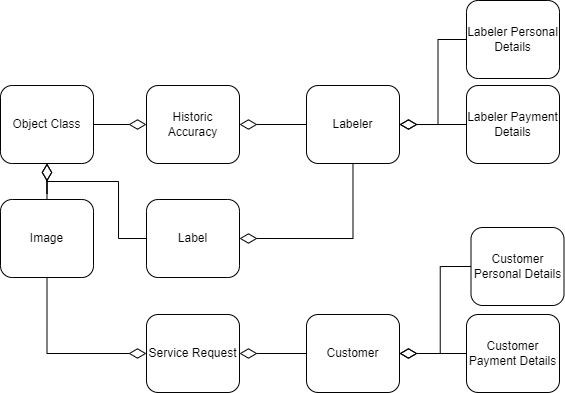
\includegraphics[scale=0.75]{businessDataModel.png}
\caption{Business Data Model}
    \label{fig:usecase}
\end{figure}
\subsection{Data Dictionary}
\begin{center}
\begin{tabular}{ |c|c|c| } % chktex 44
  \hline
    \textbf{Data Object} & \hspace{80pt} \textbf{Content} \hspace{80pt} & \textbf{Type} \\
    & & \\
    & & \\
    \hline
    Labeler &  LabelerID & Class \\ 
    \hline
    Customer &  CustomerID & Class \\ 
    \hline
    Labeler Payment Details &  LabelerID & Class \\ 
    &  Payment Details & \\
    \hline
    Customer Payment Details &  CustomerID & Class \\ 
    &  Payment Details & \\
    \hline
    Labeler Personal Details &  LabelerID & Class \\ 
    &  Personal Details & \\
    \hline
    Customer Personal Details &  CustomerID & Class \\ 
    &  Personal Details & \\
    \hline
    Historic Accuracy &  LabelerID & Class \\ 
    &  Object Class & \\
    &  Accuracy & \\
    &  Samples & \\
    \hline
    Service Request &  Image & Class \\ 
    &  CustomerID & \\
    &  Request Deadline & \\
    \hline
    Image &  Image Data & Class \\ 
    &  Image Metadata & \\
    \hline
    Label &  Labeled Class & Class \\ 
    &  Bounding Box & \\
    &  Labeler & \\
    &  Label Metadata & \\
    \hline
    Object Class &  Object Class List & Class \\ 
    &  Object Class Score & \\
    &  Labels & \\
    &  Image & \\
    \hline
    
    
\end{tabular}
\end{center}
\begin{center}
  \begin{tabular}{ |c|c|c| } % chktex 44
    \hline
    Task Allocation &  \{Service Request & Data Flow \\ 
    &  +Available Labelers & \\
    &  +Historic Accuracy & \\
    &  +Object Class & \\
    &  +Request Deadline \} & \\
    \hline
    Class Consensus &  \{Label & Data Flow \\ 
    &  +Historic Accuracy\} & \\
    \hline
    Payment Details & All details necessary to   & Attribute/Element \\ 
    & process payment. Depends on &\\
    & payment vendor and location  &  \\ 
    \hline
    Personal Details & Details necessary to identify and contact & Attribute/Element \\
    &    a user  &  \\
    \hline
    Accuracy & Represents proportion of correct labels & Attribute/Element \\
    & $a \in \mathbb{R} \wedge 0 \leq a \leq 1$ & \\
    \hline
    Samples & $n \in \mathbb{N} \wedge a \geq 0 $ & Attribute/Element \\
    \hline
    Request Deadline & YYYY-MM-DDTHH:MM:SS & Attribute/Element \\
    & In 24HR UTC &  \\
    \hline
    Image Data & NxM grid of RGB pixels & Attribute/Element \\
    \hline
    Image Metadata & Additional details related to an image& Attribute/Element \\
    \hline
    Label class & String representing class of object& Attribute/Element \\
    \hline
    Bounding Box & $(x_0,y_0),(x_1,y_1)$ where  & Attribute/Element \\
    & $\forall x_j,y_j |: 0 \leq x_j \leq N \wedge 0 \leq y_j \leq M $   &  \\
    \hline
    Label Metadata & Additional details related to an label& Attribute/Element \\
    \hline
    Object Class List & List of classes reported in image & Attribute/Element \\
    \hline
    Object Class Score & Likelihood of class appearing in image & Attribute/Element \\
    & $s \in \mathbb{R} \wedge 0 \leq s \leq 1$ &  \\
    \hline

  \end{tabular}

\end{center}
\newpage
\section{The Scope of the Product}
\subsection{Product Boundary}
The use case diagram depicted below identifies the boundaries between the users and the product.
\begin{figure}[H]
    \centering
    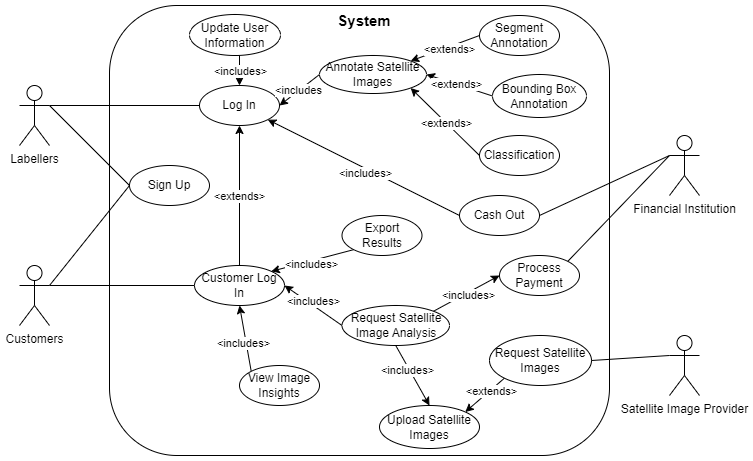
\includegraphics[scale=0.63]{useCaseDiagram.png}
    \caption{Use Case diagram}
    \label{fig:usecase}
\end{figure}
\newpage
\subsection{Product Use Case Table}
\begin{longtable}
 {p{0.1\textwidth} | p{0.35\textwidth} | p{0.2\textwidth} | p{0.35\textwidth}}
  \toprule
  \textbf{PUC No} & \textbf{PUC Name} & \textbf{Actor/s} & \textbf{Input \& Output}\\
  \midrule
  1 & Sign Up & Labelers, Customers & Personal information \& credentials (in), New account (out)\\
  \midrule
  2 & Log In & Labelers & Credentials (in)\\
  \midrule
  3 & Customer Log In & Customers & Credentials (in)\\
  \midrule
  4 & Update User Information & Labelers, Customers & Information to change (in),  Updated information (out)\\
   \midrule
  5 & Annotate Images & Labelers & Image \& annotation (in), Labeled image (out)\\
  \midrule
  6 & Segment Annotation & Labelers & Segmented image \& user selections (in), Image with labeled segments (out)\\
  \midrule
  7 & Bounding Box Annotation & Labelers & Image \& box annotations (in), Image with labeled boxes (out)\\
  \midrule
  8 & Classification & Labelers & Image \& choices (in), Image labeled with the selected choice (out)\\
  \midrule
   9 & Cash Out & Labelers, Financial Institution & Financial information (in), Payment to user (out)\\
  \midrule
  10 & View Image Insights & Customers & Request to view insights (in), Image insights (out)\\
  \midrule
  11 & Export Results & Customers & Request to export results (in), Results in downloadable format (out)\\
  \midrule
  12 & Request Image Analysis & Customers & Labels, images \& examples (in) \\
  \midrule
  13 & Upload Images & Customers & Images (in)\\
  \midrule
  14 & Request Images & Customers, Satellite Image Provider & Description of images wanted (in), Images (out)\\
  \midrule
  15 & Process Payment & Customers, Financial Institution & Financial information (in), Payment to app (out)\\
  \bottomrule
  \caption{Product Use Cases} \label{TblPUC}\\
\end{longtable}
\subsection{Individual Product Use Cases (PUC's)}
\subsubsection*{PUC0 - Sign Up}
\label{sec:PUC0}
\textbf{Primary Actors:} Labelers, Customers\\ 
\textbf{Precondition:} None\\
\textbf{Trigger:} User selects create an account\\
\textbf{Success Scenario:}
\begin{enumerate}
    \item User provides the required information and agrees with the privacy policy of the application
    \item System verifies all required information has been provided and is of valid syntax
    \item System securely registers the given information
    \item User is directed to the login page
\end{enumerate}
\textbf{Post-condition:} User has successfully created an account and the application has securely stored their information\\
\textbf{Related:} \hyperref[sec:FR0]{FR0}

\subsubsection*{PUC1 - Log In}
\label{sec:PUC1}
\textbf{Primary Actors:} Labelers\\ 
\textbf{Precondition:} Labeler has signed up for an account\\
\textbf{Trigger:} Labeler selects log in\\
\textbf{Success Scenario:}
\begin{enumerate}
    \item Labeler enters credentials
    \item System verifies all required information has been provided and matches the stored records
    \item Labeler is redirected to the home page as a logged-in user
\end{enumerate}
\textbf{Post-condition:} The labeler has access to their account. All account related information, such as labeling progress, is accurately represented\\
\textbf{Related:} \hyperref[sec:FR10]{FR10}

\subsubsection*{PUC2 - Customer Log In}
\label{sec:PUC2}
\textbf{Primary Actors:} Customers\\ 
\textbf{Precondition:} Customer has signed up for an account\\
\textbf{Trigger:} Customer selects log in\\
\textbf{Success Scenario:}
\begin{enumerate}
    \item Customer enters credentials
    \item System verifies all required information has been provided and matches the stored records
    \item Customer is redirected to the home page as a logged-in customer, which gives them access to more features than a labeler
\end{enumerate}
\textbf{Post-condition:} The customer has access to their account and all their current image analysis projects\\
\textbf{Related:} \hyperref[sec:FR1]{FR1}

\subsubsection*{PUC3 - Update User Information}
\label{sec:PUC3}
\textbf{Primary Actors:} Labelers, Customers\\ 
\textbf{Precondition:} User has logged in\\
\textbf{Trigger:} User selects update information\\
\textbf{Success Scenario:}
\begin{enumerate}
    \item User enters updated information
    \item System verifies the new information has valid syntax
    \item System updates the information
    \item User is given a confirmation that their information has been updated
\end{enumerate}
\textbf{Post-condition:} The information that the system stores about the user has been updated\\
\textbf{Related:} \hyperref[sec:FR2]{FR2}, \hyperref[sec:FR11]{FR11}

\subsubsection*{PUC4 - Annotate Satellite Images}
\label{sec:PUC4}
\textbf{Primary Actors:} Labelers\\ 
\textbf{Precondition:} Labeler has logged in\\
\textbf{Trigger:} Labeler selects a listed project\\
\textbf{Success Scenario:}
\begin{enumerate}
    \item A satellite image related to the selected project and a description of what to annotate is shown to the labeler
    \item The labeler annotates the satellite image to the best of their ability
    \item The annotated satellite image is submitted by the labeler
    \item The labeler is rewarded and the satellite image is stored by the system
    \item If the labeler skips the image rather than submits it, then the annotated image will not be stored by the system and the labeler will not receive a reward
    \item The next satellite image of the selected project is shown to the labeler and the process repeats
\end{enumerate}
\textbf{Post-condition:} All submitted annotated satellite images are stored by the system. The labeler's reward balance is updated to reflect their submissions\\
\textbf{Related:} \hyperref[sec:FR13]{FR13}

\subsubsection*{PUC5 - Segment Annotation}
\label{sec:PUC5}
\textbf{Primary Actors:} Labelers\\ 
\textbf{Precondition:} Labeler has logged in\\
\textbf{Trigger:} Labeler selects a listed project\\
\textbf{Success Scenario:}
\begin{enumerate}
    \item The same as Annotate Images, but the labeler is given a satellite image segmented into different parts and must label each segment to the best of their ability 
\end{enumerate}
\textbf{Post-condition:} All submitted annotated satellite images are stored by the system. The labeler's reward balance is updated to reflect their submissions\\
\textbf{Related:} \hyperref[sec:FR13]{FR13}

\subsubsection*{PUC6 - Bounding Box Annotation}
\label{sec:PUC6}
\textbf{Primary Actors:} Labelers\\ 
\textbf{Precondition:} Labeler has logged in\\
\textbf{Trigger:} Labeler selects a listed project\\
\textbf{Success Scenario:}
\begin{enumerate}
    \item The same as Annotate Images, but the labeler must annotate areas of the satellite image by drawing boxes and providing a label for each box
\end{enumerate}
\textbf{Post-condition:} All submitted annotated satellite images are stored by the system. The labeler's reward balance is updated to reflect their submissions\\
\textbf{Related:} \hyperref[sec:FR13]{FR13}

\subsubsection*{PUC7 - Classification}
\label{sec:PUC7}
\textbf{Primary Actors:} Labelers\\ 
\textbf{Precondition:} Labeler has logged in\\
\textbf{Trigger:} Labeler selects a listed project\\
\textbf{Success Scenario:}
\begin{enumerate}
    \item The same as Annotate Images, but the labeler must classify what category a satellite image belongs to given several options
\end{enumerate}
\textbf{Post-condition:} All submitted annotated satellite images are stored by the system. The labeler's reward balance is updated to reflect their submissions\\
\textbf{Related:} \hyperref[sec:FR13]{FR13}

\subsubsection*{PUC8 - Cash Out}
\label{sec:PUC8}
\textbf{Primary Actors:} Labelers\\
\textbf{Secondary Actor:} Financial Institution\\
\textbf{Precondition:} Labeler has logged in and their reward balance is at least \$1\\
\textbf{Trigger:} Labeler selects cash out\\
\textbf{Success Scenario:}
\begin{enumerate}
    \item The system retrieves the labeler's payment information
    \item The labeler confirms it is correct, or updates their information accordingly
    \item The system sends a payment to the labeler through their financial institution
    \item The labeler's reward balance is set back to \$0
\end{enumerate}
\textbf{Post-condition:} The financial account that the labeler provided has gained money equal to the labeler's reward balance\\
\textbf{Related:} \hyperref[sec:FR12]{FR12}

\subsubsection*{PUC9 - View Image Insights}
\label{sec:PUC9}
\textbf{Primary Actors:} Customers\\
\textbf{Precondition:} Customer has logged in and has at least one satellite image analysis project\\
\textbf{Trigger:} Customer selects insights for a project\\
\textbf{Success Scenario:}
\begin{enumerate}
    \item The system provides the customer with a progress update, key statistics, and an overview of current labels for specific satellite images
    \item The customer selects a specific image to view insights 
    \item The system gets the information it has stored related to the image and provides insights such as confidence level of annotations
\end{enumerate}
\textbf{Post-condition:} The customer has knowledge about how their project is progressing and if the labeling of the satellite images has been complete\\
\textbf{Related:} \hyperref[sec:FR5]{FR5}, \hyperref[sec:FR14]{FR14}

\subsubsection*{PUC10 - Export Results}
\label{sec:PUC10}
\textbf{Primary Actors:} Customers\\
\textbf{Precondition:} Customer has logged in, has at least one satellite image analysis project, and all labeled satellite images in that project have an acceptable accuracy\\
\textbf{Trigger:} Customer selects export data\\
\textbf{Success Scenario:}
\begin{enumerate}
    \item The system retrieves all the labeled satellite images associated with the project
    \item The system asks the customer where they would like the images to be saved
    \item The customer specifies the save location
    \item The images are downloaded to the specified location
\end{enumerate}
\textbf{Post-condition:} The customer has complete access to the labeled dataset of satellite images\\
\textbf{Related:} \hyperref[sec:FR5]{FR5}, \hyperref[sec:FR14]{FR14}

\subsubsection*{PUC11 - Request Image Analysis}
\label{sec:PUC11}
\textbf{Primary Actors:} Customers\\
\textbf{Precondition:} Customer has logged in\\
\textbf{Trigger:} Customer creates a new project request\\
\textbf{Success Scenario:}
\begin{enumerate}
    \item The system prompts the customer with a form to fill out regarding information about the project such as what is to be labeled
    \item The customer fills out the form and submits it
    \item The system confirms the forms information is valid. It prompts the customer to upload the satellite image dataset to be analyzed
    \item The customer uploads their own satellite images or requests the system to get images for them
    \item The system asks the customer to provide sample labeled images that can be shared with labelers
    \item The customer uploads sample labeled images
    \item Based on the size and difficulty of the project, the system provides the total cost of the project to the customer
    \item The customer provides their payment details
    \item The system processes the payment
    \item The system makes the project available to labelers so they can annotate the satellite images
\end{enumerate}
\textbf{Post-condition:} The image analysis project has been created and labelers can start annotating the satellite images\\
\textbf{Related:} \hyperref[sec:FR4]{FR4}

\subsubsection*{PUC12 - Upload Satellite Images}
\label{sec:PUC12}
\textbf{Primary Actors:} Customers\\
\textbf{Precondition:} Customer has logged in and has created a new project request\\
\textbf{Trigger:} Customer submits the information form for a new project\\
\textbf{Success Scenario:}
\begin{enumerate}
    \item The system prompts the customer to upload the images they would like to be analyzed
    \item The customer selects the images they want analyzed and uploads them
    \item The system stores the images with a reference to the project
\end{enumerate}
\textbf{Post-condition:} The system has all the images that will be analyzed for the project\\
\textbf{Related:} \hyperref[sec:FR6]{FR6}

\subsubsection*{PUC13 - Request Satellite Images}
\label{sec:PUC13}
\textbf{Primary Actors:} Customers\\
\textbf{Secondary Actors:} Satellite Image Provider\\
\textbf{Precondition:} Customer has logged in and has created a new project request\\
\textbf{Trigger:} Customer submits the information form for a new project\\
\textbf{Success Scenario:}
\begin{enumerate}
    \item The system prompts the customer about the type of satellite images they want. This could be satellite images from a specific time frame in a specific area
    \item The customer specifies the type of satellite images they want for analysis
    \item The system contacts a satellite image provider, and pays a fee to them in exchange for the images. The fee is charged to the customer
    \item The system stores the images with a reference to the project
\end{enumerate}
\textbf{Post-condition:} The system has all the satellite images that will be analyzed for the project\\
\textbf{Related:} \hyperref[sec:FR7]{FR7}

\subsubsection*{PUC14 - Process Payment}
\label{sec:PUC14}
\textbf{Primary Actors:} Customers\\
\textbf{Secondary Actor:} Financial Institution\\
\textbf{Precondition:} Customer has logged in and has created a new project request\\
\textbf{Trigger:} Customer has filled out all the details of the project and uploaded all the photos\\
\textbf{Success Scenario:}
\begin{enumerate}
    \item The system retrieves the customer's payment information
    \item The customer confirms it is correct, or updates their information accordingly
    \item The system sends a payment request to the customer's financial institution
    \item The financial institution validates the payment information and sends the payment
    \item The payment is deposited in the financial account associated with the system
\end{enumerate}
\textbf{Post-condition:} The fees for facilitating the project have been paid\\
\textbf{Related:} \hyperref[sec:FR3]{FR3}

\subsection*{Context Diagram}
\begin{figure}[H]
  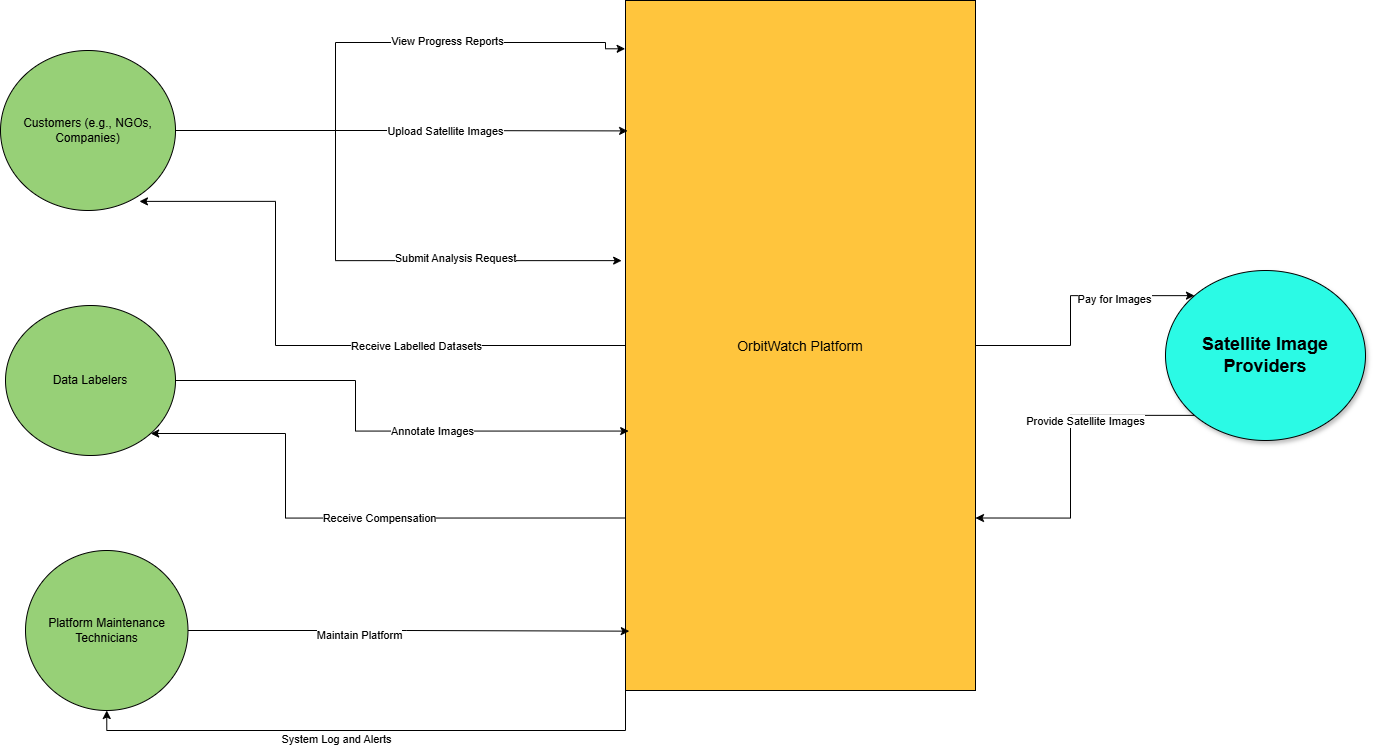
\includegraphics[scale=0.3]{contextdiagram.png}
  \caption{Context Diagram}
      \label{fig:context}
  \end{figure}

\newpage
\section{Functional Requirements}
\subsection{Functional Requirements}
\subsubsection*{FR0}
\label{sec:FR0}
\begin{itemize}
  \item \textbf{Description:} The system shall allow Customers to create a new user account.
  \item \textbf{Rationale:} The customers must have an account to request the services provided by the system.
  \item \textbf{Fit Criterion:} Customer is created in and stored in the database.
  \item \textbf{Related:} \hyperref[sec:PUC0]{PUC0}, \hyperref[sec:PR0]{NFR-PR0}, \hyperref[sec:SE2]{NFR-SE2}
\end{itemize}
\subsubsection*{FR1}
\label{sec:FR1}
\begin{itemize}
  \item \textbf{Description:} The system shall allow customers with an existing account to authenticate themselves using the credentials stored by the system.
  \item \textbf{Rationale:} To access privileged information, the system must authenticate customers.
  \item \textbf{Fit Criterion:} Customer can use correct credentials to log in to user account.
  \item \textbf{Related:} \hyperref[sec:PUC2]{PUC2}, \hyperref[sec:SE1]{NFR-SE1}
\end{itemize}
\subsubsection*{FR2}
\label{sec:FR2}
\begin{itemize}
  \item \textbf{Description:} The system shall allow authenticated Customers to edit their account information.
  \item \textbf{Rationale:} After creating an account, the customers must have the necessary tools to modify the information they have provided.
  \item \textbf{Fit Criterion:} After logging in, customers can modify the stored personal information.
  \item \textbf{Related:} \hyperref[sec:PUC3]{PUC3}, \hyperref[sec:UH0]{NFR-UH0}
\end{itemize}
\subsubsection*{FR3}
\label{sec:FR3}
\begin{itemize}
  \item \textbf{Description:} The system shall accept payments from authenticated Customers.
  \item \textbf{Rationale:} To request services, the system shall integrate with payment services.
  \item \textbf{Fit Criterion:} After logging in, customers can send a payment to the system.
  \item \textbf{Related:} \hyperref[sec:PUC14]{PUC14}, \hyperref[sec:OE2]{NFR-OE2}, \hyperref[sec:SE9]{NFR-SE9}
\end{itemize}
\subsubsection*{FR4}
\label{sec:FR4}
\begin{itemize}
  \item \textbf{Description:} The system shall accept service requests from authenticated Customers.
  \item \textbf{Rationale:} The system’s key offering is the ability to request services.
  \item \textbf{Fit Criterion:} After logging in, customers can send a service request which is accepted by the system.
  \item \textbf{Related:} \hyperref[sec:PUC11]{PUC11}, \hyperref[sec:PR7]{NFR-PR7}, \hyperref[sec:SE1]{NFR-SE1}
\end{itemize}
\subsubsection*{FR5}
\label{sec:FR5}
\begin{itemize}
  \item \textbf{Description:} The system shall provide reports to authenticated customers when a service request is complete.
  \item \textbf{Rationale:} The system must provide the results of a service request to the users who initiated it.
  \item \textbf{Fit Criterion:} After logging in and after the completion of a service request, customers can receive a service request report.
  \item \textbf{Related:} \hyperref[sec:PUC9]{PUC9}, \hyperref[sec:PUC10]{PUC10}, \hyperref[sec:PR2]{NFR-PR2}
\end{itemize}
\subsubsection*{FR6}
\label{sec:FR6}
\begin{itemize}
  \item \textbf{Description:} The system shall allow an authenticated Customer to upload images associated with a service request.
  \item \textbf{Rationale:} If the customer has images to be analyzed, they must have the ability to upload them to the system.
  \item \textbf{Fit Criterion:} After logging in and after the initiation of a service request, customers can add images associated to the service request.
  \item \textbf{Related:} \hyperref[sec:PUC12]{PUC12}, \hyperref[sec:PR8]{NFR-PR8}
\end{itemize}
\subsubsection*{FR7}
\label{sec:FR7}
\begin{itemize}
  \item \textbf{Description:} The system shall allow a customer to request satellite images for a given geographic area, as designated using a specified geographic coordinate system.
  \item \textbf{Rationale:} If customers do not have images for the area they would like to be analyzed, they can request the system to source them on their behalf. They system may not be able to fulfill the request.
  \item \textbf{Fit Criterion:} After logging in and after the initiation of a service request, customers can request the system to locate images from external providers by providing geographic coordinates.
  \item \textbf{Related:} \hyperref[sec:PUC13]{PUC13}, \hyperref[sec:PR8]{NFR-PR8}, \hyperref[sec:OE1]{NFR-OE1}
\end{itemize}
\subsubsection*{FR8}
\label{sec:FR8}
\begin{itemize}
  \item \textbf{Description:} The system shall alert a customer if their service request is not able to be fulfilled.
  \item \textbf{Rationale:} In the event the system is unable to complete a request, it should alert the customer, so they are aware.
  \item \textbf{Fit Criterion:} After logging in and after the initiation of a service request, the customer will get an alert if the request in unable to be fufiled.
  \item \textbf{Related:} \hyperref[sec:SE4]{NFR-SE4}
\end{itemize}
\subsubsection*{FR9}
\label{sec:FR9}
\begin{itemize}
  \item \textbf{Description:} The system shall allow Labelers to create a new user account.
  \item \textbf{Rationale:} The Labelers must have an account to request the services provided by the system.
  \item \textbf{Fit Criterion:} Labeler is created in and stored in the database.
  \item \textbf{Related:} \hyperref[sec:PUC0]{PUC0}, \hyperref[sec:PR1]{NFR-PR1}, \hyperref[sec:SE2]{NFR-SE2}, \hyperref[sec:SE3]{NFR-SE3}
\end{itemize}
\subsubsection*{FR10}
\label{sec:FR10}
\begin{itemize}
  \item \textbf{Description:} The system shall allow Labelers with an existing account to authenticate themselves using the credentials stored by the system.
  \item \textbf{Rationale:} In order to access privileged information, the system must Labelers customers.
\item \textbf{Fit Criterion:} Labelers can use correct credentials to log in to user account.
\item \textbf{Related:} \hyperref[sec:PUC1]{PUC1}, \hyperref[sec:SE0]{NFR-SE0}
\end{itemize}
\subsubsection*{FR11}
\label{sec:FR11}
\begin{itemize}
  \item \textbf{Description:} The system shall allow authenticated Labelers to edit their account information.
  \item \textbf{Rationale:} After creating an account, the Labelers must have the necessary tools to modify the information they have provided.
  \item \textbf{Fit Criterion:} After logging in, Labelers can modify the stored personal information.
  \item \textbf{Related:}  \hyperref[sec:PUC4]{PUC4}, \hyperref[sec:UH0]{NFR-UH0}
\end{itemize}
\subsubsection*{FR12}
\label{sec:FR12}
\begin{itemize}
  \item \textbf{Description:} The system shall allow Labelers to request their accrued earnings be transferred to their provided banking platform.
  \item \textbf{Rationale:} The system must ensure Labelers are compensated for their efforts.
\item \textbf{Fit Criterion:} After logging in, Labelers can request their earnings be deposited in the account stored in their personal information.
\item \textbf{Related:}  \hyperref[sec:PUC8]{PUC8}, \hyperref[sec:PR4]{NFR-PR4}, \hyperref[sec:OE2]{NFR-OE2}, \hyperref[sec:SE9]{NFR-SE9}
\end{itemize}
\subsubsection*{FR13}
\label{sec:FR13}
\begin{itemize}
  \item \textbf{Description:} The system shall allow Labelers to annotate images displayed to them with the purpose of collecting annotation data.
  \item \textbf{Rationale:} This is the key service the system provides.
  \item \textbf{Fit Criterion:} Labelers will be able to annotate images.
  \item \textbf{Related:} \hyperref[sec:PUC4]{PUC4}, \hyperref[sec:PUC5]{PUC5}, \hyperref[sec:PUC6]{PUC6}, \hyperref[sec:PUC7]{PUC7}, \hyperref[sec:UH2]{NFR-UH2}, \hyperref[sec:UH9]{NFR-UH9} \hyperref[sec:PR3]{NFR-PR3}, \hyperref[sec:SE0]{NFR-SE0}
\end{itemize}
\subsubsection*{FR14}
\label{sec:FR14}
\begin{itemize}
  \item \textbf{Description:} The system shall combine annotations obtained from authenticated Labelers into a consolidated report.
  \item \textbf{Rationale:} This is the key service the system provides.
  \item \textbf{Fit Criterion:} After a service request has been initaited, and the system has determined the label accuracy is over a certain threshold.
  \item \textbf{Related:} \hyperref[sec:PUC9]{PUC9}, \hyperref[sec:PUC10]{PUC10} \hyperref[sec:PR5]{NFR-PR5}
\end{itemize}

\newpage
\subsection{Traceability}
\setlength\LTleft{-2cm}
\scriptsize
\begin{longtable}{l|ccccccccccccccc}

PUC \# & \multicolumn{15}{c}{Functional Requirement} \\ \hline
\endfirsthead
%
\endhead
%
 & \hyperref[sec:FR0]{FR0} & \hyperref[sec:FR1]{FR1} & \hyperref[sec:FR2]{FR2} & \hyperref[sec:FR3]{FR3} & \hyperref[sec:FR4]{FR4} & \hyperref[sec:FR5]{FR5} & \hyperref[sec:FR6]{FR6} & \hyperref[sec:FR7]{FR7} & \hyperref[sec:FR8]{FR8} & \hyperref[sec:FR9]{FR9} & \hyperref[sec:FR10]{FR10} & \hyperref[sec:FR11]{FR11} & \hyperref[sec:FR12]{FR12} & \hyperref[sec:FR13]{FR13} & \hyperref[sec:FR14]{FR14} \\
\hyperref[sec:PUC0]{PUC0} & X &  &  &  &  &  &  &  &  & X &  &  &  &  &  \\
\hyperref[sec:PUC1]{PUC1} &  &  &  &  &  &  &  &  &  &  & X &  &  &  &  \\
\hyperref[sec:PUC2]{PUC2} &  & X &  &  &  &  &  &  &  &  &  &  &  &  &  \\
\hyperref[sec:PUC3]{PUC3} &  &  & X &  &  &  &  &  &  &  &  & X &  &  &  \\
\hyperref[sec:PUC4]{PUC4} &  &  &  &  &  &  &  &  &  &  &  &  &  & X &  \\
\hyperref[sec:PUC5]{PUC5} &  &  &  &  &  &  &  &  &  &  &  &  &  & X &  \\
\hyperref[sec:PUC6]{PUC6} &  &  &  &  &  &  &  &  &  &  &  &  &  & X &  \\
\hyperref[sec:PUC7]{PUC7} &  &  &  &  &  &  &  &  &  &  &  &  &  & X &  \\
\hyperref[sec:PUC8]{PUC8} &  &  &  &  &  &  &  &  &  &  &  &  & X &  &  \\
\hyperref[sec:PUC9]{PUC9} &  &  &  &  &  & X &  &  &  &  &  &  &  &  & X \\
\hyperref[sec:PUC10]{PUC10} &  &  &  &  &  & X &  &  &  &  &  &  &  &  & X \\
\hyperref[sec:PUC11]{PUC11} &  &  &  &  & X &  &  &  &  &  &  &  &  &  &  \\
\hyperref[sec:PUC12]{PUC12} &  &  &  &  &  &  & X &  &  &  &  &  &  &  &  \\
\hyperref[sec:PUC13]{PUC13} &  &  &  &  &  &  &  & X &  &  &  &  &  &  &  \\
\hyperref[sec:PUC14]{PUC14} &  &  &  & X &  &  &  &  &  &  &  &  &  &  & \\
\caption{Traceability between FR and PUC} \\
\end{longtable}

\setlength\LTleft{-2cm}
\begin{longtable}{l|ccccccccccccccc}

NFR \# & \multicolumn{15}{c}{Functional Requirement} \\ \hline
\endfirsthead
%
\endhead
%
 & \hyperref[sec:FR0]{FR0} & \hyperref[sec:FR1]{FR1} & \hyperref[sec:FR2]{FR2} & \hyperref[sec:FR3]{FR3} & \hyperref[sec:FR4]{FR4} & \hyperref[sec:FR5]{FR5} & \hyperref[sec:FR6]{FR6} & \hyperref[sec:FR7]{FR7} & \hyperref[sec:FR8]{FR8} & \hyperref[sec:FR9]{FR9} & \hyperref[sec:FR10]{FR10} & \hyperref[sec:FR11]{FR11} & \hyperref[sec:FR12]{FR12} & \hyperref[sec:FR13]{FR13} & \hyperref[sec:FR14]{FR14} \\
\hyperref[sec:UH0]{UH0} &  &  & X &  &  &  &  &  &  &  &  & X &  &  &  \\
\hyperref[sec:UH2]{UH2} &  &  &  &  &  &  &  &  &  &  &  &  &  & X &  \\
\hyperref[sec:UH9]{UH9} &  &  &  &  &  &  &  &  &  &  &  &  &  & X &  \\
\hyperref[sec:PR0]{PR0} & X &  &  &  &  &  &  &  &  &  &  &  &  &  &  \\
\hyperref[sec:PR1]{PR1} &  &  &  &  &  &  &  &  &  & X &  &  &  &  &  \\
\hyperref[sec:PR2]{PR2} &  &  &  &  &  & X &  &  &  &  &  &  &  &  &  \\
\hyperref[sec:PR3]{PR3} &  &  &  &  &  &  &  &  &  &  &  &  &  & X &  \\
\hyperref[sec:PR4]{PR4} &  &  &  &  &  &  &  &  &  &  &  &  & X &  &  \\
\hyperref[sec:PR5]{PR5} &  &  &  &  &  &  &  &  &  &  &  &  &  &  & X \\
\hyperref[sec:PR7]{PR7} &  &  &  &  & X &  &  &  &  &  &  &  &  &  &  \\
\hyperref[sec:PR8]{PR8} &  &  &  &  &  &  & X & X &  &  &  &  &  &  &  \\
\hyperref[sec:OE1]{OE1} &  &  &  &  &  &  &  & X &  &  &  &  &  &  &  \\
\hyperref[sec:OE2]{OE2} &  &  &  & X &  &  &  &  &  &  &  &  & X &  &  \\
\hyperref[sec:SE0]{SE0} &  &  &  &  &  &  &  &  &  &  & X &  &  & X &  \\
\hyperref[sec:SE1]{SE1} &  & X &  &  & X &  &  &  &  &  &  &  &  &  &  \\
\hyperref[sec:SE2]{SE2} & X &  &  &  &  &  &  &  &  & X &  &  &  &  &  \\
\hyperref[sec:SE3]{SE3} & X &  &  &  &  &  &  &  &  & X &  &  &  &  &  \\
\hyperref[sec:SE4]{SE4} &  &  &  &  &  &  &  &  & X &  &  &  &  &  &  \\
\hyperref[sec:SE9]{SE9} &  &  &  & X &  &  &  &  &  &  &  &  & X &  & \\
\caption{Traceability between FR and NFR} \\
\end{longtable}

\normalsize

\section{Look and Feel Requirements}
\subsection{Appearance Requirements}
\subsubsection*{NFR-LF0}
\label{sec:LF0}
\begin{itemize}
  \item \textbf{Description:} The application shall adapt to various screen sizes, ensuring legibility and an uncluttered layout.
  \item \textbf{Rationale:} Users will have computers with varying screen sizes, so a consistent experience across all these sizes is ideal.
  \item \textbf{Fit Criterion:} Visual elements must not exceed the boundaries of a screen with a size between the range 1024×768 pixels to 1920×1080 pixels.
\end{itemize}
\subsubsection*{NFR-LF1}
\label{sec:LF1}
\begin{itemize}
  \item \textbf{Description:} Interactive elements such as buttons shall provide visual feedback to the user.
  \item \textbf{Rationale:} This will allow users a better understanding of when their actions have been processed by the application.
  \item \textbf{Fit Criterion:} Every interactive element changes colour or displays additional visual cues, such as animations or shadows, to indicate interaction.
\end{itemize}
\subsection{Style Requirements}
\subsubsection*{NFR-LF2}
\label{sec:LF2}
\begin{itemize}
  \item \textbf{Description:} The application should maintain a unified visual design across all components.
  \item \textbf{Rationale:} A consistent appearance enhances the application's cohesiveness and conveys a professional aesthetic.
  \item \textbf{Fit Criterion:} Font type, sizing, and colour, along with background tones are all consistent throughout the application.
\end{itemize}

\section{Usability and Humanity Requirements}

\subsection{Ease of Use Requirements}



\subsubsection*{NFR-UH0}
\label{sec:UH0}
      \begin{itemize}
          \item \textbf{Description}: The platform will have a well-organized navigation menu, allowing users to quickly find labeling tasks, settings, help, and account details.  
          \item \textbf{Rationale}: An easy-to-navigate platform helps reduce the time taken for users to find what they need, improving the efficiency of labeling tasks and overall user satisfaction.  
          \item \textbf{Fit Criterion}: At least 90\% of users should be able to navigate to any main feature within 3 clicks, as determined by usability testing.
          \item \textbf{Related:} \hyperref[sec:FR2]{FR2}, \hyperref[sec:FR11]{FR11}
      \end{itemize}
\subsubsection*{NFR-UH1}
\label{sec:UH1}
      \begin{itemize}
          \item \textbf{Description}: The platform’s buttons, forms, and other UI elements should follow a consistent style and behavior throughout, to ensure a predictable user experience.  
          \item \textbf{Rationale}: Consistency reduces cognitive load and helps users feel comfortable and confident when interacting with the system, as they can easily recognize and understand patterns in the UI.  
          \item \textbf{Fit Criterion}: Consistency will be validated by usability tests where at least 95\% of users recognize and correctly use recurring interface elements across different pages.
      \end{itemize}


\subsection{Personalization and Internationalization Requirements}


\subsubsection*{NFR-UH2} 
\label{sec:UH2}
        \begin{itemize}
            \item \textbf{Description}: Users can set preferences to prioritize specific types of labeling tasks (e.g., agricultural, urban) and receive suggestions aligned with their interests and expertise.  
            \item \textbf{Rationale}: Allowing users to work on tasks of interest or within their expertise can improve task accuracy and user satisfaction, leading to better retention and data quality.  
            \item \textbf{Fit Criterion}: Users should be able to set their task preferences in their profile, with at least 80\% of their assigned tasks matching these preferences over time.
            \item \textbf{Related:} \hyperref[sec:FR13]{FR13}
        \end{itemize}
        \subsubsection*{NFR-UH3} 
        \label{sec:UH3}
        \begin{itemize}
            \item \textbf{Description}: The platform should display localized formats for date, time, and currency based on the user's location or preference settings.  
            \item \textbf{Rationale}: Displaying culturally familiar formats enhances user comfort and reduces errors when interpreting critical information like deadlines or earnings.  
            \item \textbf{Fit Criterion}: Date, time, and currency formats should adjust automatically based on the user’s location or manual settings, verified through localized testing.
        \end{itemize}


\subsection{Learning Requirements}


\subsubsection*{NFR-UH4} 
\label{sec:UH4}
        \begin{itemize} 
            \item \textbf{Description}: Users can track their progress through tutorials and training tasks within the platform, allowing them to see completed and pending learning modules.  
            \item \textbf{Rationale}: Tracking progress motivates users to complete learning tasks and helps them understand where they stand in terms of mastering platform features.  
            \item \textbf{Fit Criterion}: A progress tracker will be implemented, and at least 80\% of users should find it helpful, based on post-training feedback surveys.
        \end{itemize}
        \subsubsection*{NFR-UH5} 
        \label{sec:UH5}
        \begin{itemize} 
            \item \textbf{Description}: Provide users with simulated labeling tasks to practice without affecting actual datasets, allowing them to learn through hands-on experience before starting real work.  
            \item \textbf{Rationale}: Practice tasks help users understand the labeling process without pressure, improving their confidence and accuracy before handling real data.  
            \item \textbf{Fit Criterion}: At least 85\% of users should complete at least one practice task before labeling real data, with a satisfaction rate of 90\% based on feedback.
        \end{itemize}


\subsection{Understandability and Politeness Requirements}


\subsubsection*{NFR-UH6} 
\label{sec:UH6}
        \begin{itemize} 
            \item \textbf{Description}: Contextual help pop-ups should be available throughout the platform, offering brief explanations for various features and guidance on how to complete tasks.  
            \item \textbf{Rationale}: Providing help exactly where users need it reduces confusion and makes it easier for users to understand how to use different parts of the platform without extensive searching.  
            \item \textbf{Fit Criterion}: At least 90\% of users should find the contextual help pop-ups clear and helpful during usability testing.
        \end{itemize}
        \subsubsection*{NFR-UH7} 
        \label{sec:UH7}
        \begin{itemize} 
            \item \textbf{Description}: Error messages will not only indicate what went wrong but also provide actionable steps to resolve the issue in a friendly, non-blaming tone.  
            \item \textbf{Rationale}: Friendly and constructive error handling reduces user frustration and helps users quickly resolve issues without needing support, improving overall experience.  
            \item \textbf{Fit Criterion}: At least 95\% of errors will be accompanied by actionable instructions, and users should report a low frustration rate ($<$ 10\%) when encountering errors, based on feedback.
        \end{itemize}


\subsection{Accessibility Requirements}


\subsubsection*{NFR-UH8} 
\label{sec:UH8}
        \begin{itemize} 
            \item \textbf{Description}: The platform will provide options for users to adjust text size and choose between different color themes (e.g., light, dark, high contrast) to improve readability based on their preferences.  
            \item \textbf{Rationale}: Allowing adjustments for visual elements helps users with low vision, color blindness, or different environmental lighting conditions to comfortably use the platform.  
            \item \textbf{Fit Criterion}: At least three different color themes will be available, and users should be able to increase text size up to 200\% without loss of content or functionality.
        \end{itemize}
        \subsubsection*{NFR-UH9} 
        \label{sec:UH9}
        \begin{itemize} 
            \item \textbf{Description}: The platform will support keyboard shortcuts for essential actions (e.g., navigating between tasks, submitting labels) to facilitate quick access and improve usability for users who cannot use a mouse.  
            \item \textbf{Rationale}: Keyboard shortcuts provide an alternative way to interact with the system, improving efficiency for power users and ensuring accessibility for users with limited mobility.  
            \item \textbf{Fit Criterion}: All core actions should have keyboard shortcuts available, and usability tests should confirm that at least 95\% of actions are accessible via keyboard navigation.
            \item \textbf{Related:} \hyperref[sec:FR13]{FR13}
        \end{itemize}



\section{Performance Requirements}
\subsection{Speed and Latency Requirements}
\subsubsection*{NFR-PR0}
\label{sec:PR0}
\begin{itemize}
  \item \textbf{Description:} The system shall process new user requests within 15 minutes of a Customer completing the account creation process 90\% of the time, and within 48 hours in all cases. 
  \item \textbf{Rationale:} The user likely has urgent needs if they are signing up to access the system. They must have quick access to the services offered by the system, and authentication is the first step of this process.
  \item \textbf{Fit Criterion:}\\ Let $t_{\text{newCustomerAccount}}$ be the time it takes to process a new Customer account request, in hours.\\ \probP($t_{\text{newCustomerAccount}} < 0.25) \geq .90 \wedge \probP(t_{\text{newCustomerAccount}} < 48) = 1 $
  \item \textbf{Related:} \hyperref[sec:FR0]{FR0}
\end{itemize}

\subsubsection*{NFR-PR1}
\label{sec:PR1}
\begin{itemize}
  \item \textbf{Description:} The system shall process new user requests within 15 minutes of a Labeler  completing the account creation process 90\% of the time, and within 48 hours in all cases. 
  \item \textbf{Rationale:} To improve engagement from Labelers, there should be minimal delay in getting started.
  \item \textbf{Fit Criterion:}\\ Let $t_{\text{newLabelAccount}}$ be the time it takes to process a new Labeler account request, in hours.\\ \probP($t_{\text{newLabelAccount}} < 0.25) \geq 0.9 \wedge \probP(t_{\text{newLabelAccount}} < 48) = 1 $
  \item \textbf{Related:} \hyperref[sec:FR9]{FR9}
\end{itemize}

\subsubsection*{NFR-PR2}
\label{sec:PR2}
\begin{itemize}
  \item \textbf{Description:} The system shall return a complete report of results to the Customer within the negotiated amount of time, 90\% of the time, and within 48 additional hours in all cases.
  \item \textbf{Rationale:} The user is expecting to be able to act on the insights the system provides. To build trust and loyalty, the system must ensure that it is meeting the agreed upon timelines.
  \item \textbf{Fit Criterion:}\\ Let $t_{\text{serviceRequestTime}}$ be the time it takes to complete a service request, in hours.\\
  Let $t_{\text{serviceRequestTimeLimit}}$ be the negotiated time limit for completing a service request, in hours.\\ \probP($t_{\text{serviceRequestTime}} < t_{\text{serviceRequestTimeLimit}}) \geq 0.9\\ \wedge \probP(t_{\text{serviceRequestTime}} < t_{\text{serviceRequestTimeLimit}}+48) = 1 $
  \item \textbf{Related:} \hyperref[sec:FR5]{FR5},  \hyperref[sec:PR7]{NFR-PR7}
\end{itemize}

\subsubsection*{NFR-PR3}
\label{sec:PR3}
\begin{itemize}
  \item \textbf{Description:} The system shall take no longer than 10 seconds to display the next image to be labeled to a labeler, if there is one available.
  \item \textbf{Rationale:} To reduce friction for labelers, the system must ensure there is no unnecessary delay in preparing the next job. For users exposed to modern media, attention spans can be expected to be less than 10 seconds \href{https://profiletree.com/attention-span-crisis-digital-age-statistics/#:~:text=Studies%20have%20proven%20that%20being,focus%20after%208%20mere%20seconds}{src}.
  \item \textbf{Fit Criterion:}\\ Let $t_{\text{imageServing}}$ be the time it takes to serve the next image, in seconds.\\
  Let $x_{\text{nextImage}}$ equal True if there is a next image available, and False otherwise.\\
  $x_{\text{nextImage}} \Rightarrow t_{\text{imageServing}} \leq 10$
  \item \textbf{Related:} \hyperref[sec:FR13]{FR13}
\end{itemize}

\subsubsection*{NFR-PR4}
\label{sec:PR4}
\begin{itemize}
  \item \textbf{Description:} The system shall deliver earned payouts to labelers within 7 business days of a request being made through the system.
  \item \textbf{Rationale:} The labelers are entitled to their earned income, and there must not be unnecessary delay. 7 days accounts for delays in the platform used to distribute payments.
  \item \textbf{Fit Criterion:}\\ Let $t_{\text{payoutDelay}}$ be the time it takes for a user to receive their payments after a request is received by the system, in days.\\
  $t_{\text{payoutDelay}} < 7$
  \item \textbf{Related:} \hyperref[sec:FR12]{FR12}
\end{itemize}
\subsection{Safety-Critical Requirements}
N/A
\subsection{Precision or Accuracy Requirements}
\subsubsection*{NFR-PR5}
\label{sec:PR5}
\begin{itemize}
  \item \textbf{Description:} The system shall report accurate labels 75\% of the time.
  \item \textbf{Rationale:} Average data label accuracy for competitors is greater than 75\% (\href{https://www.researchgate.net/publication/234774537_Data_quality_from_crowdsourcing_A_study_of_annotation_selection_criteria#:~:text=Depending%20on%20the%20number%20of,%5B13%5D%20%5B14%5D%20.}{link}). The system should at a minimum provide the same label accuracy.
  \item \textbf{Fit Criterion:}\\ Let $O$ be the set of objects to label.\\
  Let $C$ be the set of classes an object in $O$ can be.\\
  Let $L_{\text{True}}: O \rightarrow C $ be a function which maps objects in $O$ to their true classes in $C$.
  Let $L_{\text{Guess}}: O \rightarrow C $ be the funtion derived from the system which maps objects in $O$ to their assumed classes in $C$.
  $(\forall o \in O|: \probP(L_{\text{True}}(o) = L_{\text{Guess}}(o))\geq 0.75)$
  \item \textbf{Related:} \hyperref[sec:FR14]{FR14}
\end{itemize}
\subsection{Robustness or Fault-Tolerance Requirements}
\subsubsection*{NFR-PR6}
\label{sec:PR6}
\begin{itemize}
  \item \textbf{Description:} The system shall have 97\% uptime. 
  \item \textbf{Rationale:} It is crucial that in emergency response use cases, the system is able to accept and process requests with minimal delay.
  \item \textbf{Fit Criterion:}\\ Let $t_{\text{uptime}}$ be the uptime of the system.\\
  Let $t_{\text{downtime}}$ be the downtime of the system.\\
  $\frac{t_{\text{uptime}}}{t_{\text{uptime}} + t_{\text{downtime}}} > 0.97$
\end{itemize}
\subsection{Capacity Requirements}
\subsubsection*{NFR-PR7}
\label{sec:PR7}
\begin{itemize}
  \item \textbf{Description:} The system shall have the capacity to support enough labelers to meet all service request deadlines.
  \item \textbf{Rationale:} This requirement is critical to satisfy NFR-PR2.
  \item \textbf{Fit Criterion:} See \hyperref[sec:PR2]{NFR-PR2}.
  \item \textbf{Related:} \hyperref[sec:FR4]{FR4},  \hyperref[sec:PR2]{NFR-PR2},  \hyperref[sec:PR9]{NFR-PR9}
\end{itemize}
\subsubsection*{NFR-PR8}
\label{sec:PR8}
\begin{itemize}
  \item \textbf{Description:} The system shall have the capacity to store and process large image files.
  \item \textbf{Rationale:} This requirement is necessary to obtain information from satelite images, which can be several gigabites in size.
  \item \textbf{Fit Criterion:} The system will not crash or fail to store when given images files <50 Gb in size.
  \item \textbf{Related:} \hyperref[sec:FR6]{FR6}, \hyperref[sec:FR7]{FR7}
\end{itemize}
\subsection{Scalability or Extensibility Requirements}
\subsubsection*{NFR-PR9}
\label{sec:PR9}
\begin{itemize}
  \item \textbf{Description:} The system shall be able to scale to meet the capacity specified in NFR-PR7.
  \item \textbf{Rationale:} This requirement is critical to satisfy NFR-PR7.
  \item \textbf{Fit Criterion:} See \hyperref[sec:PR7]{NFR-PR7}.
   \item \textbf{Related:} \hyperref[sec:PR7]{NFR-PR7}
\end{itemize}
\subsection{Longevity Requirements}
N/A


\section{Operational and Environmental Requirements}
\subsection{Expected Physical Environment}
N/A
\subsection{Wider Environment Requirements}
% \subsubsection{Sustainability}
\subsubsection*{NFR-OE0}
\label{sec:OE0}
\begin{itemize}
  \item \textbf{Description:} The system shall implement energy-efficient practices in cloud usage and server management.
  \item \textbf{Rationale:} Minimizes the platform’s carbon footprint and promotes sustainability.
  \item \textbf{Fit Criterion:} Cloud infrastructure usage is optimized to reduce energy consumption by at least 20\% compared to baseline measurements.
\end{itemize}
\subsection{Requirements for Interfacing with Adjacent Systems}
\subsubsection*{NFR-OE1}
\label{sec:OE1}
\begin{itemize}
  \item \textbf{Description:} The system shall support standardized APIs and data formats for the automatic acquisition and integration of satellite images from third-party providers.
  \item \textbf{Rationale:} Facilitates seamless integration and efficient data handling from satellite data providers.
  \item \textbf{Fit Criterion:} The platform can successfully ingest data from at least two major satellite data providers using their APIs without manual intervention.
  \item \textbf{Related:} \hyperref[sec:FR7]{FR7}
\end{itemize}
\subsubsection*{NFR-OE2}
\label{sec:OE2}
\begin{itemize}
  \item \textbf{Description:} The system shall integrate with reliable and secure payment processors to handle user compensations and client payments efficiently.
  \item \textbf{Rationale:} Ensures secure and efficient financial transactions, building trust with users and clients.
  \item \textbf{Fit Criterion:} Transactions are processed securely through integrated payment gateways, achieving a transaction success rate of 99.5%.
  \item \textbf{Related:} \hyperref[sec:FR3]{FR3}, \hyperref[sec:FR12]{FR12}
\end{itemize}
\subsubsection*{NFR-OE3}
\label{sec:OE3}
\begin{itemize}
  \item \textbf{Description:} The system shall support multiple currencies to accommodate a global user base and international clients.
  \item \textbf{Rationale:} Enhances the platform’s accessibility and usability for users and clients worldwide.
  \item \textbf{Fit Criterion:} The platform supports at least four major currencies (e.g., USD, EUR, GBP, INR) and correctly processes transactions in each.
\end{itemize}
\subsubsection*{NFR-OE4}
\label{sec:OE4}
\begin{itemize}
  \item \textbf{Description:} The system shall be compatible with popular machine learning frameworks to facilitate the training, testing, and deployment of computer vision models.
  \item \textbf{Rationale:} Enables efficient development and integration of ML models for various use cases.
  \item \textbf{Fit Criterion:} The platform can train and deploy models using frameworks like TensorFlow, PyTorch, and scikit-learn without compatibility issues.
\end{itemize}
\subsubsection*{NFR-OE5}
\label{sec:OE5}
\begin{itemize}
  \item \textbf{Description:} The system shall have efficient data pipelines for transferring labeled datasets between the platform and ML models.
  \item \textbf{Rationale:} Ensures smooth and automated workflows for data handling and model training.
  \item \textbf{Fit Criterion:} Data transfers occur within minutes, and pipelines support batch processing of large datasets (e.g., 10,000 images) without errors.
\end{itemize}
\subsection{Productization Requirements}
\subsubsection*{NFR-OE6}
\label{sec:OE6}
\begin{itemize}
  \item \textbf{Description:} The system shall be accessible without requiring any installation, operating solely through web browsers.
  \item \textbf{Rationale:} Eliminates the need for users to install software, reducing barriers to entry and simplifying access.
  \item \textbf{Fit Criterion:} Users can access and use the platform by visiting the web URL on any supported browser without needing to download or install additional software.
\end{itemize}
\subsection{Release Requirements}
\subsubsection*{NFR-OE7}
\label{sec:OE7}
\begin{itemize}
  \item \textbf{Description:} The system shall include a detailed release roadmap outlining timelines, features, and milestones for upcoming releases.
  \item \textbf{Rationale:} Keeps the development team and stakeholders aligned and ensures organized progress.
  \item \textbf{Fit Criterion:} The release roadmap is documented, updated regularly, and adhered to with at least 80\% of milestones achieved on schedule.
\end{itemize}
\subsubsection*{NFR-OE8}
\label{sec:OE8}
\begin{itemize}
  \item \textbf{Description:} The system shall be showcased to select group of users to gather feedback, identify bugs, and refine features before full-scale deployment.
  \item \textbf{Rationale:} Ensures the platform meets user expectations and operates smoothly upon official release.
  \item \textbf{Fit Criterion:} Testing results in fewer than 10 critical bugs identified and includes actionable feedback from at least 50 labelers, leading to necessary iterative improvements.
\end{itemize}
\subsubsection*{NFR-OE9}
\label{sec:OE9}
\begin{itemize}
  \item \textbf{Description:} Each release shall preserve the core functionality of existing features without introducing regressions or deprecations.
  \item \textbf{Rationale:} Ensures continuity and reliability of the platform by preventing new updates from disrupting or breaking previously working features, thereby maintaining user trust and satisfaction.
  \item \textbf{Fit Criterion:} Automated usability testing is performed for each release, and no existing critical features fail post-release. Verification is achieved through passing all regression test cases before deployment.
\end{itemize}


\section{Maintainability and Support Requirements}
\subsection{Maintenance Requirements}
\subsubsection*{NFR-MR0}
\label{sec:MR0}
\begin{itemize}
  \item \textbf{Description:} All maintainance required for the system shall be possible to complete by a competent software developer after reading all of the documentation provided in the source repository.
  \item \textbf{Rationale:} The system should be well documented, and therefore maintainable after reading said documents.
  \item \textbf{Fit Criterion:} A competent software developer, as determined by the original developers or their agents, can solve problems related to the core of the system, as determined by the 
  features outlined in this document.
\end{itemize}
\subsection{Supportability Requirements}
N/A
\subsection{Adaptability Requirements}
N/A

\section{Security Requirements}
\subsection{Access Requirements}
\subsubsection*{NFR-SE0}
\label{sec:SE0}
\begin{itemize}
  \item \textbf{Description:} The application shall only allow users with labeling access, including labellers, customers, and admins, to view active projects and label images.
  \item \textbf{Rationale:} We do not want random users with no stake in the process to effect the results.
  \item \textbf{Fit Criterion:} Users who have not logged in to the application have no way of viewing projects or labeling images. Users logged in as labellers, customers, or admins have access to these features.
  \item \textbf{Related:} \hyperref[sec:FR10]{FR10}, \hyperref[sec:FR13]{FR13}
\end{itemize}
\subsubsection*{NFR-SE1}
\label{sec:SE1}
\begin{itemize}
  \item \textbf{Description:} The application shall only allow users with customer access and above to create new image analysis projects.
  \item \textbf{Rationale:} Unidentified users creating projects would be impossible to facilitate. Also, labellers have no need to access project creation. 
  \item \textbf{Fit Criterion:} Users who have not logged in to the application have no way of creating an image analysis project. Users logged in as customers or admins have access to these features.
  \item \textbf{Related:} \hyperref[sec:FR1]{FR1}, \hyperref[sec:FR4]{FR4}
\end{itemize}
\subsubsection*{NFR-SE2}
\label{sec:SE2}
\begin{itemize}
  \item \textbf{Description:} The application shall validate the email format the user provides when creating an account.
  \item \textbf{Rationale:} We do not want users using invalid or duplicate emails to sign up.
  \item \textbf{Fit Criterion:} Let E represent the set of all email addresses, and let V represent the set of all valid email addresses. A valid email address conforms to the general pattern:\\\\
  V = $(\forall\; email \in E\;  |\; email \; matches \; the \; pattern \; $[a-zA-Z0-9+\_.-]+@[a-zA-Z0-9.-]+[a-zA-Z])\\
  $\text{New email} \in V \land \text{New email} \neg \in \text{Registered Emails}$
  \item \textbf{Related:}  \hyperref[sec:FR0]{FR0}, \hyperref[sec:FR9]{FR9}
\end{itemize}
\subsubsection*{NFR-SE3}
\label{sec:SE3}
\begin{itemize}
  \item \textbf{Description:} The application shall validate the password format the user provides when creating an account.
  \item \textbf{Rationale:} We do not want users using weak passwords to sign up.
  \item \textbf{Fit Criterion:} Let P represent the set of all passwords, and let V represent the set of all valid passwords. A valid password has a at least one lowercase, uppercase, number and special character and is a minimum of 8 characters in length:\\\\
  V = $(\forall\; password \in P\;  |\; password \; matches \; the \; pattern \; $(?=.*[a-z])(?=.*[A-Z])(?=.*[0-9])(?=.*[\#\$\%\&\*\@])[a-zA-Z0-9\#\$\%\&\*\@]\{8,\})\\
  \item \textbf{Related:} \hyperref[sec:FR0]{FR0}, \hyperref[sec:FR9]{FR9}
\end{itemize}
\subsubsection*{NFR-SE4}
\label{sec:SE4}
\begin{itemize}
  \item \textbf{Description:} The system shall, during system failure, notify users trying to make a request of the system failure.
  \item \textbf{Rationale:} The system should provide good warning messages to users to prevent additional frustration.
  \item \textbf{Fit Criterion:} When services are unavailable, the system shall provide an error message to the user making the request of the unavailable service.
  \item \textbf{Related:} \hyperref[sec:FR8]{FR8}
\end{itemize}
\subsection{Integrity Requirements}
\subsubsection*{NFR-SE5}
\label{sec:SE5}
\begin{itemize}
  \item \textbf{Description:} The application shall prevent incorrect data from being introduced.
  \item \textbf{Rationale:} The database of information should always reflect correct and up to date information.
  \item \textbf{Fit Criterion:} The system must validate user inputs for data accuracy and format before they are saved. Any invalid data must trigger error messages, preventing it from being entered into the database. Users must be required to correct errors before proceeding.
\end{itemize}
\subsubsection*{NFR-SE6}
\label{sec:SE6}
\begin{itemize}
  \item \textbf{Description:} The application shall prohibit new user actions when user is disconnected from the system.
  \item \textbf{Rationale:} The system should avoid batch updates upon reconnect as to prevent malicious users creating a false package of updates.
  \item \textbf{Fit Criterion:} Upon user disconnect and reconnect, the system will not accept any updates from the user not submitted before the disconnect occured.
\end{itemize}
\subsubsection*{NFR-SE7}
\label{sec:SE7}
\begin{itemize}
  \item \textbf{Description:} The system shall reject duplicate entries in database.
  \item \textbf{Rationale:} Each entry to the database should be a unique data piece. If two entries are identical, they must differ by at least the creation time.
  \item \textbf{Fit Criterion:} No two entries in the database shall exist together for longer than 24 hours from their introduction into the database.
\end{itemize}
\subsection{Privacy Requirements}
\subsubsection*{NFR-SE8}
\label{sec:SE8}
\begin{itemize}
  \item \textbf{Description:} User data will be securely encrypted to protect user’s privacy.
  \item \textbf{Rationale:} This will help to avoid user's being compromised if a data leak occurs.
  \item \textbf{Fit Criterion:} An encryption algorithm is used on sensitive user data such as passwords.
\end{itemize}
\subsubsection*{NFR-SE9}
\label{sec:SE9}
\begin{itemize}
  \item \textbf{Description:} The application shall ensure that all payment transactions are processed securely using encryption and comply with relevant security standards, such as PCI-DSS, which helps to protect payment account data (PCI Security Standards Council, 2024).
  \item \textbf{Rationale:} Protecting users' financial information is critical to maintaining trust. Failing to secure payments can lead to data breaches, financial loss, and legal liabilities.
  \item \textbf{Fit Criterion:} All payment transactions must use industry-standard encryption to protect sensitive data. Payment information, such as credit card details, must not be stored locally on the application and must be processed via a secure, PCI-DSS-compliant third-party payment gateway.
  \item \textbf{Related:} \hyperref[sec:FR3]{FR3}, \hyperref[sec:FR12]{FR12}
\end{itemize}

\subsection{Audit Requirements}
N/A
\subsection{Immunity Requirements}
\subsubsection*{NFR-SE10}
\label{sec:SE10}
\begin{itemize}
  \item \textbf{Description:} The application shall use parameterized queries or prepared statements for all database interactions.
  \item \textbf{Rationale:} We want to prevent SQL injection attacks which can lead to unauthorized data access or manipulation.
  \item \textbf{Fit Criterion:} All database queries must be implemented using parameterized queries or prepared statements. Dynamic SQL strings that concatenate user input must not be used in the codebase.
\end{itemize}

\section{Cultural Requirements}
\subsection{Cultural Requirements}
\subsubsection*{NFR-CU0}
\label{sec:CU0}
\begin{itemize}
  \item \textbf{Description:} The system shall present users with the option to select the most popular language in each country it is deployed in.
  \item \textbf{Rationale:} It is important that the users of the program can understand what is said in each step.
  \item \textbf{Fit Criterion:} A drop down will allow users to select from the list of languages. At a minimum, the most popular language by number of speakers will be available for each country.
\end{itemize}

\section{Compliance Requirements}
\subsection{Legal Requirements}
\subsubsection*{NFR-CO0}
\label{sec:CO0}
\begin{itemize}
  \item \textbf{Description:} The system shall not be available in any country currently facing economic sanctions by the Government of Canada.
  \item \textbf{Rationale:} Legal requirement to operate.
  \item \textbf{Fit Criterion:} Website must not be reachable in sanctioned countries. Canadian sanctions are outlined in the following legislation: \href{http://laws-lois.justice.gc.ca/eng/acts/U-2/index.html}{United Nation Act}, \href{http://laws-lois.justice.gc.ca/eng/acts/S-14.5/index.html}{Special Economic Measures Act}, and \href{http://laws.justice.gc.ca/eng/acts/J-2.3/}{Justice for Victims of Corrupt Foreign Officials Act}
\end{itemize}
\subsubsection*{NFR-CO1}
\label{sec:CO1}
\begin{itemize}
  \item \textbf{Description:} The system shall follow Canadian tax code when accepting and paying out earnings.
  \item \textbf{Rationale:} Legal requirement to operate.
  \item \textbf{Fit Criterion:} All relevant tax codes must be satisfied when accepting payment from Customers or paying out earnings to Labelers. Specifically \href{https://www.ontario.ca/laws/statute/90c40}{Ontario Tax Act, 1990} and \href{https://laws-lois.justice.gc.ca/eng/acts/i-3.3/}{Income Tax Act 1985}
\end{itemize}
\subsubsection*{NFR-CO2}
\label{sec:CO2}
\begin{itemize}
  \item \textbf{Description:} The system shall allow Customers to restrict Labelers from certain regions from labeling the images related to their service request.
  \item \textbf{Rationale:} Customers may be uploading sensitive images, which are inappropriate for international Labelers to view.
  \item \textbf{Fit Criterion:} No restricted image, as identified by the customer, shall be shown to a restricted group.
\end{itemize}
\subsection{Standards Compliance Requirements}
N/A

\section{Open Issues}
\textbf{Task Assignment Algorithm: }To ensure labelers are engaged as they complete tasks and to obtain the highest quality of information possible, the system must implement an intelligent task allocation system. This system has not yet been determined.
\\\textbf{Label Consensus Algorithm: }Similarly, the algorithm for combining multiple user labels into one accurate label has not yet been determined. 
\\\textbf{Labeling Services Offered: }The system has determined several potential labeling services to be offered by the system, but has not confirmed with certainty what will be included. This will be determined after more research has been completed on the task assignment algorithm.

\section{Off-the-Shelf Solutions}
\subsection{Ready-Made Products}
\textbf{Amazon Mechanical Turk: } A web-based crowdsourcing platform. Instead of building a novel front end, the system could obtain labels through this platform instead.
\subsection{Reusable Components}
\textbf{Label Studio: } A React library which contains components for building a web-based data annotation platform.
\subsection{Products That Can Be Copied}
\textbf{Toloka AI: } A general purpose image label crowdsourcing site. Supports image segmentation, bounding box drawing, and more computer vision labeling tasks. \href{https://toloka.ai/}{Toloka.ai}



\section{New Problems}
\subsection{Effects on the Current Environment}
The introduction of the OKKM Insights platform is expected to have several impacts on the existing technological and operational environment.
\subsubsection{Data Privacy and Security Concerns}
\begin{enumerate}
    \item Impact: Handling sensitive satellite imagery and user-generated data raises significant privacy and security issues. Ensuring compliance with data protection regulations is most important.
    \item Potential Problem: Breaches or mishandling of data could lead to legal repercussions, loss of trust, and reputational damage.
\end{enumerate}
\subsubsection{Environmental Footprint}
\begin{enumerate}
    \item Impact: Increased computational requirements for AI processing and data storage may lead to higher energy consumption.
    \item Potential Problem: This could conflict with sustainability goals and lead to higher operational costs.
\end{enumerate}
\subsection{Effects on the Installed Systems}
Introducing the OKKM Insights platform will interact with and potentially disrupt existing systems within the organization and for stakeholders.
\subsubsection{Integration Challenges}
\begin{enumerate}
    \item Impact: The platform will need to integrate with existing data sources, cloud services, and possibly applicable third-party APIs.
    \item Potential Problem: Incompatibilities or integration failures could result in data inconsistencies, system downtimes, or increased maintenance efforts.
\end{enumerate}
\subsubsection{Legacy Systems Compatibility}
\begin{enumerate}
    \item Impact: Older systems may not support the latest technologies required by the new platform.
    \item Potential Problem: Upgrading or adjusting to legacy systems can be costly and time-consuming, potentially delaying the platform's deployment.
\end{enumerate}
\subsection{Potential User Problems}
Users are at the heart of the OKKM Insights platform, and several issues may arise that affect their experience and satisfaction.
\subsubsection{Usability Issues}
\begin{enumerate}
    \item Impact: If the platform is not intuitive or user-friendly, users may struggle to navigate and utilize its features effectively.
    \item Potential Problem: Poor user experience can lead to reduced engagement, lower data labeling contributions, and higher dropout rates.
\end{enumerate}
\subsubsection{Training and Onboarding}
\begin{enumerate}
    \item Impact: Users may require training to understand how to label data accurately and use the platform's tools.
    \item Potential Problem: Inadequate training resources can result in inconsistent labeling, decreasing the quality of the datasets and the reliability of the AI models.
\end{enumerate}
\subsubsection{Compensation and Incentives}
\begin{enumerate}
    \item Impact: Users expect fair compensation for their contributions.
    \item Potential Problem: Delays or inaccuracies in payment processing can lead to dissatisfaction, reducing user retention and the overall quality of data labeling efforts.
\end{enumerate}
\subsubsection{Technical Support}
\begin{enumerate}
    \item Impact: Users may encounter technical issues that require timely resolution.
    \item Potential Problem: Insufficient support can frustrate users, leading to decreased platform usage and negative word-of-mouth.
\end{enumerate}
\subsection{Limitations in the Anticipated Implementation Environment That May
Inhibit the New Product}
Several environmental and contextual limitations could hinder the effective implementation and operation of the OKKM Insights platform.
\subsubsection{Regulatory Constraints}
\begin{enumerate}
    \item Limitation: Different countries have varying regulations regarding satellite data usage, privacy, and AI applications.
    \item Impact: Navigating these regulatory landscapes can be complex and may restrict the platform's operations in certain regions, limiting market potential.
\end{enumerate}
\subsubsection{Technological Dependencies}
\begin{enumerate}
    \item Limitation: The platform relies on third-party services (e.g., cloud providers, satellite data suppliers) whose availability and reliability are beyond the project's control.
    \item Impact: Downtime or changes in third-party services can disrupt platform functionality and user experience.
\end{enumerate}
\subsection{Follow-Up Problems}
Addressing the initial set of problems may give rise to additional challenges that need to be managed.
\subsubsection{Data Quality Management}
\begin{enumerate}
    \item Follow-Up Problem: Ensuring the ongoing accuracy and relevance of labeled datasets as new data is continuously added. This may require implementing robust quality assurance mechanisms and periodic reviews.
\end{enumerate}
\subsubsection{User Engagement and Retention}
\begin{enumerate}
    \item Follow-Up Problem: Continuously engaging users to maintain an active labeling workforce may require ongoing incentives, gamification strategies, and community-building efforts to prevent user fatigue and attrition.
\end{enumerate}
\subsubsection{Ethical Considerations}
\begin{enumerate}
    \item Follow-Up Problem: Addressing ethical concerns related to surveillance, data misuse, and the potential dual-use nature of satellite imagery data. Establishing ethical guidelines and oversight mechanisms will be necessary to prevent misuse.
\end{enumerate}
\subsubsection{Dependency on User Participation}
\begin{enumerate}
    \item Follow-Up Problem: The platform's success heavily relies on active user participation for data labeling. Changes in user engagement can directly impact data quality and availability, requiring strategies to stabilize user contributions.
\end{enumerate}
\subsubsection{Technical Debt Accumulation}
\begin{enumerate}
    \item Follow-Up Problem: Rapid development to address emerging problems may lead to technical debt, where short-term solutions create long-term maintenance challenges. Proper code management and refactoring practices will be needed to mitigate this issue.
\end{enumerate}



\section{Tasks}

\subsection{Project Planning}
\begin{itemize} 
    \item \textbf{Define Clear Milestones}: Establish milestones based on key project phases, such as requirements gathering, hazard analysis, proof of concept, backend development, and final project demonstration.
    \item \textbf{Task Assignment and Role Allocation}: Assign tasks to team members based on their strengths and expertise, with clear ownership over specific deliverables (e.g., backend development, frontend development, documentation, testing).
    \item \textbf{Use of Project Management Tools}: Utilize tools like Kanban boards in GitHub Projects to track progress, organize tasks into 'To Do,' 'In Progress,' and 'Completed' categories, and set internal deadlines to meet project milestones effectively.
    \item \textbf{Risk Management and Mitigation}: Identify potential project risks (e.g., data quality issues, development delays) and create mitigation strategies, including regular check-ins, backup plans, and prioritization of critical tasks.
\end{itemize}

\subsection{Planning of the Development Phases}
\begin{itemize} 
    \item \textbf{Requirements Gathering (24-Sep-2024 to 08-Oct-2024)}: Engage in detailed discussions with stakeholders to gather comprehensive requirements for both frontend and backend components, ensuring all technical and business needs are documented.
    \item \textbf{Hazard Analysis (10-Oct-2024 to 23-Oct-2024)}: Identify risks related to data handling, server security, and other critical project components. Develop a hazard analysis document to mitigate potential threats, especially in handling satellite imagery.
    \item \textbf{Verification \& Validation (V\&V) Planning (24-Oct-2024 to 01-Nov-2024)}: Develop a detailed V\&V plan, including test plans and quality assurance measures. This will include setting up testing environments and criteria for ensuring code correctness and reliability.
    \item \textbf{Proof of Concept (01-Nov-2024 to 22-Nov-2024)}: Develop basic functionality for both backend and frontend, demonstrating image processing, API development, and the labeling workflow. Gather feedback to identify areas of improvement.
    \item \textbf{Backend Development (23-Nov-2024 to 05-Jan-2025)}: Focus on developing API endpoints, integrating satellite image data, and ensuring secure and efficient handling of large datasets. Aim to have a functional backend by the end of this phase.
    \item \textbf{Frontend Development (23-Nov-2024 to 05-Jan-2025)}: Design and implement UI/UX features, integrate backend APIs, and ensure an interactive user experience for both clients and labelers. Aim for a fully functional frontend that complements backend capabilities.
    \item \textbf{Design Document Revision (15-Dec-2024 to 15-Jan-2025)}: Revise the design document to reflect final system architecture, covering database schema, API structure, and AI model integration.
    \item \textbf{Mid-Project Demonstration (03-Feb-2025 to 14-Feb-2025)}: Prepare a functional prototype showcasing the integrated backend, frontend, and APIs. Demonstrate the labeling process, data flow, and key system functionalities.
    \item \textbf{Verification \& Validation (15-Feb-2025 to 07-Mar-2025)}: Test data processing pipelines, system reliability, and user interfaces to ensure accuracy and consistency. Run automated and manual tests for different use cases.
    \item \textbf{Final Project Demonstration \& Expo Preparation (24-Mar-2025 to 01-Apr-2025)}: Demonstrate the complete system, including all functionality, datasets, and models. Fine-tune UI and prepare for a polished presentation at the Expo.
    \item \textbf{Final Documentation (01-Apr-2025 to 15-Apr-2025)}: Compile comprehensive final reports covering the entire development process, technical documentation, user manuals, and deployment guides.
\end{itemize}

\section{Migration to the New Product}
\subsection{Requirements for Migration to the New Product}
N/A
\subsection{Data That Has to be Modified or Translated for the New System}
N/A

\section{Costs}
Developing and implementing the requirements for the OKKM Insights platform involves various financial and effort-related expenditures. 
    Below is a detailed breakdown of the primary cost components associated with building the platform:

\subsection{Development Costs}
\subsubsection{Software Development}
\begin{enumerate}
    \item Front-End Development: Creating a user-friendly web interface requires experience working with front-end technologies such as HTML, CSS, JavaScript, and frameworks like React or Angular.
    \item Back-End Development: Developing robust server-side infrastructure using technologies like Node.js, Flask, and Python. This includes setting up databases, APIs, and integrating with cloud services (AWS/Azure).
    \item AI and Machine Learning Integration: Building and integrating AI-powered features for automatic data labeling and computer vision model training will require specialized expertise in machine learning, potentially increasing development costs.
  \end{enumerate}
\subsubsection{UI/UX Design}
\begin{enumerate}
  \item Investing time into UI/UX design to ensure the platform is intuitive and easy to use for both data labelers and end clients. This includes designing workflows, views, and ensuring responsive design across devices.
  \end{enumerate}
  \subsubsection{Testing and Quality Assurance}
\begin{enumerate}
  \item Comprehensive testing to identify and fix bugs, ensure cross-platform compatibility, and maintain high system reliability. This involves both automated and manual testing processes.
  \end{enumerate}
\subsection{Infrastructure Costs}
\subsubsection{Cloud Services}
\begin{enumerate}
  \item Hosting: Utilizing cloud platforms like AWS or Azure for hosting the backend services and databases. Costs will scale with usage, including storage for satellite images, computational resources for AI processing, and data transfer fees.
  \item Scalability: Ensuring the infrastructure can scale to handle increasing numbers of users and data volume, which may involve additional costs for load balancing, auto-scaling, and enhanced security measures.
  \end{enumerate}
\subsubsection{Data Acquisition}
\begin{enumerate}
  \item Purchasing high-quality, commercially available satellite images from third-party providers. These costs can vary based on the resolution, coverage area, and frequency of image updates required for different use cases.
  \end{enumerate}
\subsection{Operational Costs}
\subsubsection{User Compensation}
\begin{enumerate}
  \item Labeling Incentives: Allocating funds to compensate users who contribute to the image labeling process. This includes setting competitive rates to attract and retain a large and active user base.
  \item Payment Processing Fees: Costs associated with handling financial transactions, including fees from payment gateways for distributing earnings to users and receiving payments from clients.
  \end{enumerate}
\subsubsection{Maintenance and Support}
\begin{enumerate}
  \item Ongoing maintenance of the platform to ensure uptime, implement updates, and address technical issues. This also includes providing customer support to both data labelers and end clients.
  \end{enumerate}
\subsubsection{Security and Compliance}
\begin{enumerate}
  \item Implementing robust security measures to protect sensitive satellite data and financial transactions. Costs may include encryption technologies, regular security audits, and compliance with data protection regulations.
  \end{enumerate}

\subsection{Marketing and User Acquisition Costs}
\subsubsection{Promotional Activities}
\begin{enumerate}
  \item Marketing efforts to attract both data labelers and end clients to the platform. This includes digital marketing campaigns, partnerships with relevant organizations, and participation in industry events.
  \end{enumerate}
\subsubsection{Onboarding and Training}
\begin{enumerate}
  \item Creating tutorials, documentation, and training materials to facilitate easy onboarding of new users and ensure they can effectively contribute to the labeling process with minimal friction.
  \end{enumerate}

\subsection{Contingency and Miscellaneous Costs}
\subsubsection{Unexpected Expenses}
\begin{enumerate}
  \item Allocating a budget for unforeseen challenges such as technical setbacks, additional feature requests, or changes in market conditions that may require pivoting the project strategy.
  \end{enumerate}

\subsection{Budget Forecast}
A detailed budget forecast will be developed, encompassing all the aforementioned cost categories. This forecast will be periodically reviewed and adjusted based on project milestones, market conditions, and actual expenditure patterns to ensure financial sustainability and efficient resource allocation.



\section{User Documentation and Training}

\subsection{User Documentation Requirements}

        \subsubsection*{NFR-UD0} 
        \label{sec:UD0}
        \begin{itemize} 
            \item \textbf{Description}: A built-in help system with a searchable knowledge base, FAQs, tutorial videos, user forums and step-by-step guides to assist users with common issues or tasks directly within the platform.  
            \item \textbf{Rationale}: An online help system provides quick, on-demand support, improving user experience by minimizing interruptions when seeking assistance.  
            \item \textbf{Fit Criterion}: At least 80\% of users should be able to resolve their issues using the help system without contacting support, as validated by user surveys and support metrics.
        \end{itemize}
        \subsubsection*{NFR-UD1}
        \label{sec:UD1}
        \begin{itemize} 
            \item \textbf{Description}: A condensed guide offering a quick overview of key platform features and essential workflows to get users started rapidly.  
            \item \textbf{Rationale}: A quick start guide enables new users to become productive immediately without needing to read extensive documentation, improving their onboarding experience.  
            \item \textbf{Fit Criterion}: At least 80\% of new users should report the quick start guide as helpful, and they should be able to complete a basic labeling task within 15 minutes of using it.
        \end{itemize}
        \subsubsection*{NFR-UD2}
        \label{sec:UD2}
        \begin{itemize} 
            \item \textbf{Description}: Provide contextual help directly within the platform, such as tooltips and small info pop-ups, offering real-time guidance for features or form fields as users interact with them.  
            \item \textbf{Rationale}: In-app help reduces the learning curve and provides timely support without requiring users to leave the page or workflow they are on.  
            \item \textbf{Fit Criterion}: At least 88\% of users should find in-app help intuitive and accurate in providing the necessary support as validated by user surveys.
        \end{itemize}


\subsection{Training Requirement}


\subsubsection*{NFR-TR0}
        \label{sec:TR0}
        \begin{itemize} 
            \item \textbf{Description}: An onboarding tutorial guiding users through key platform functions interactively, offering tooltips and prompts to familiarize them with core workflows.  
            \item \textbf{Rationale}: Interactive onboarding accelerates learning, reduces user frustration, and ensures that new users can quickly perform tasks confidently.  
            \item \textbf{Fit Criterion}: At least 85\% of users should complete the onboarding tutorial successfully within 20 minutes, with a 80\% rate of positive feedback on its effectiveness.
        \end{itemize}
        \subsubsection*{NFR-TR1}
        \label{sec:TR1}
        \begin{itemize} 
            \item \textbf{Description}: A sandbox environment allowing users to practice labeling tasks without affecting live data, including quizzes and exercises to assess understanding and improve skills.  
            \item \textbf{Rationale}: A practice environment enables users to build confidence and hone their skills in a low-pressure setting, ensuring they are prepared for real tasks.  
            \item \textbf{Fit Criterion}: At least 80\% of new users should utilize the practice environment, with self-assessment scores indicating an average improvement of 20\% in labeling accuracy over their first three attempts.
        \end{itemize}



\section{Waiting Room}
N/A

\section{Ideas for Solution}

\begin{itemize} 
    \item \textbf{AI-Driven Labeling System}: Implement a machine learning model for preliminary image analysis to assist human labelers. This AI system can automatically pre-label sections of satellite images, allowing human labelers to validate or adjust these labels, significantly speeding up the process.
    
    \item \textbf{Gamification for Crowdsourced Labeling}: Introduce a gamification element to motivate and engage users who are labeling data. This can include earning points, badges, or rewards for completing labeling tasks accurately and efficiently, which can improve data quality and increase participation.
    
    \item \textbf{Intelligent Task Allocation}: Utilize an algorithm that matches labeling tasks with users based on their experience, preferences, and performance history. This ensures that difficult tasks are assigned to more experienced users while simpler tasks are made available to beginners.
    
    \item \textbf{Real-Time Collaboration and Consensus Model}: Allow multiple labelers to work on the same image in parallel, using a consensus model to determine the most accurate labels. Incorporate a review mechanism to resolve discrepancies and ensure that the final labeled data meets the required quality standards.
    
    \item \textbf{Automated Quality Assurance (QA) and Feedback}: Develop a QA system that automatically checks the quality of labeled data by comparing it to known benchmarks or running cross-validation with multiple labelers. Provide labelers with instant feedback to help improve their accuracy over time.
    
    \item \textbf{Modular Web-Based Platform Architecture}: Build a modular architecture for the platform, separating the frontend, backend, and AI components. This will allow easy updates, scalability, and the ability to add new features or services without disrupting existing functionality.
    
    \item \textbf{Flexible API for Client and User Integration}: Create an API that allows clients to easily upload satellite imagery, retrieve labeled data, and interact with the system programmatically. Also, provide endpoints for labelers to claim tasks, submit work, and check their progress or earnings.
    
    \item \textbf{Visualization Dashboard for Data Insights}: Provide clients with a dynamic dashboard that visualizes key insights derived from the labeled satellite imagery. This dashboard can display analytics, progress on labeling tasks, model accuracy, and any actionable insights relevant to the client’s industry.
    
    \item \textbf{Secure Payment and Compensation System}: Implement a secure and transparent payment system that allows clients to pay for labeled data and compensates labelers based on their contributions. Use automated transaction management to ensure timely and accurate payments to all users.
    
    \item \textbf{Cross-Platform Compatibility and Accessibility}: Design the platform to be fully accessible across devices (desktop, mobile, tablets) and compliant with accessibility standards (e.g., WCAG). This ensures that a wide range of users, including those with disabilities, can participate in labeling and use the platform effectively.
\end{itemize}

\newpage{}
\section*{References}
\begin{enumerate}
    \item Government of Canada. (2017). \textit{Government of Canada – Justice for Victims of Corrupt Foreign Officials Act}. https://laws.justice.gc.ca/eng/acts/J-2.3/
    \item Government of Canada. (1992). \textit{Government of Canada – Special Economic Measures Act}. https://laws-lois.justice.gc.ca/eng/acts/S-14.5/index.html
    \item Government of Canada. (1985). \textit{Government of Canada – Income Tax Act (1985)}. https://laws-lois.justice.gc.ca/eng/acts/i-3.3/
    \item Government of Canada. (1985). \textit{Government of Canada – United Nations Act}. https://laws-lois.justice.gc.ca/eng/acts/U-2/index.html
    \item Government of Ontario. (1990). \textit{Government of Ontario – Corporations Tax Act (1990)}. https://www.ontario.ca/laws/statute/90c40
    \item PCI Security Standards Council. (2024, May 13). \textit{PCI Security Standards Council – Protect Payment Data with Industry-driven Security Standards, Training, and Programs}. https://www.pcisecuritystandards.org/standards/pci-dss/
\end{enumerate}

\newpage{}
\section*{Appendix --- Reflection}

The information in this section will be used to evaluate the team members on the
graduate attribute of Lifelong Learning.  Please answer the following questions:

\begin{enumerate}
  \item What knowledge and skills will the team collectively need to acquire to
  successfully complete this capstone project?  Examples of possible knowledge
  to acquire include domain specific knowledge from the domain of your
  application, or software engineering knowledge, mechatronics knowledge or
  computer science knowledge.  Skills may be related to technology, or writing,
  or presentation, or team management, etc.  You should look to identify at
  least one item for each team member.
  \item For each of the knowledge areas and skills identified in the previous
  question, what are at least two approaches to acquiring the knowledge or
  mastering the skill?  Of the identified approaches, which will each team
  member pursue, and why did they make this choice?
\end{enumerate}

\textbf{Knowledge and Skills}

\textbf{Knowledge}
\begin{itemize}
    \item \textbf{Machine Learning Algorithms}: Understanding various machine learning algorithms, including supervised and unsupervised learning techniques, deep learning models, and their applications in satellite imagery analysis.
    \item \textbf{Model Evaluation and Tuning}: Gaining insights into model evaluation metrics (e.g., accuracy, precision, recall, F1 score) and techniques for hyperparameter tuning (e.g., grid search, random search, and Bayesian optimization) to improve model performance.
\end{itemize}

\textbf{Skill}
\begin{itemize}
    \item \textbf{Data Handling and Preprocessing}: Developing skills in data preprocessing techniques such as data cleaning, normalization, augmentation, and handling missing values, which are crucial for preparing satellite imagery data for analysis.
    \item \textbf{Model Deployment}: Learning the practices of deploying machine learning models in production environments, including REST APIs and containerization using Docker.
\end{itemize}

\textbf{Approaches to Acquire Knowledge and Master Skills}

\begin{itemize}
    \item \textbf{Online Courses}:
    \begin{itemize}
        \item Enroll in comprehensive online courses focused on machine learning, such as:
        \begin{itemize}
            \item \textit{“Machine Learning” by Andrew Ng} (Coursera): Covers foundational concepts, algorithms, and applications of machine learning.
            \item \textit{“Deep Learning Specialization” by Andrew Ng} (Coursera): Provides in-depth knowledge of neural networks and their applications in image processing.
            \item \textit{“Machine Learning Crash Course” by Google}: A fast-paced, practical introduction to machine learning, featuring a series of lessons relating to ML models, data, and applications of ML.
        \end{itemize}
    \end{itemize}
    
    \item \textbf{Practical Projects}:
    \begin{itemize}
        \item Engage in hands-on projects that allow us to apply machine learning concepts to satellite imagery, such as:
        \begin{itemize}
            \item Participating in \textit{Kaggle competitions} that involve image classification or object detection in satellite images.
            \item Collaborating with the team to develop a prototype of the labeling platform that incorporates real-time model predictions.
        \end{itemize}
    \end{itemize}
\end{itemize}

\textbf{Chosen Approach}

I, Kartik, will primarily pursue \textbf{online courses} to build a strong theoretical foundation in machine learning, supplemented by \textbf{practical projects} to reinforce my learning through application. This combination enables me to understand complex machine learning concepts and apply them effectively to the capstone project, ensuring the team leverages cutting-edge techniques for analyzing satellite imagery.

I, Kyle, am currently enrolled in Fundamentals of Machine Learning, Data-Driven Algorithms for Sequential Decision making, and Mathematical statistics. These courses will supplement the techniques Kartik described to help me learn the background knowledge required for the task allocation part of our project. I forsee that being the biggest challenge, but I am very excited to work on it. While taking these courses, I also have access to the professors, who will likely be willing to discuss issues we run into while designing our algorithms.

I, Mathew, will focus on completing \textbf{online courses} to get a better understanding of the basics of machine learning. Specifically, I plan to follow google's machine learning crash course. This is because it combines video lectures with interactive visuals and practice exercises, which I think is an effective way to quickly gain knowledge on a topic.
\end{document}
